\documentclass[10pt]{beamer}
\usepackage[latin1]{inputenc}
\usepackage{amsmath}
\usepackage{amssymb}
\usepackage{graphics}
\usepackage{graphicx}
\usepackage{epsfig}
\usepackage{fancyhdr}
\usepackage{wasysym}
\usepackage{latexsym}
\usepackage{amsfonts}
\usepackage{subfigure}
\usepackage{color}
\usepackage[numbers]{natbib}
\usepackage{framed}
\usepackage{multirow}
\usepackage{booktabs}
\usepackage{chngpage}
\usepackage{caption}
\usepackage{tikz}
\usepackage{mdwlist}
\usepackage{algorithm}
\usepackage{algorithmicx}
\usepackage[noend]{algpseudocode}



\DeclareMathOperator*{\argmax}{arg\,max}
\newcommand{\todo}[1]{\textcolor{red}{\textbf{TODO:} #1}}
\newcommand{\setD}{\ensuremath{D} }
\newcommand{\setW}{\ensuremath{V} }
\newcommand{\setC}{\ensuremath{C} }
\newcommand{\matD}{\ensuremath{\mathrm{D}} }
\newcommand{\matW}{\ensuremath{\mathrm{W}} }
\newcommand{\matC}{\ensuremath{\mathrm{C}} }
\newcommand{\vecdi}[1]{\ensuremath{\mathrm{v}^{D}_{#1}}}
\newcommand{\vecwi}[1]{\ensuremath{\mathrm{v}^{W}_{#1}}}
\newcommand{\vecci}[1]{\ensuremath{\mathrm{v}^{C}_{#1}}}
\newcommand{\con}{$(w_{t-c}, \ldots, w_{t-1}, w_{t+1}, \ldots, w_{t+c})$}
\newcommand{\wgt}[1]{\ensuremath{\lambda_{#1}}}
\newcommand{\traindata}{\ensuremath{\mathcal{T}}}
\newcommand{\db}{\ensuremath{\mathcal{D}} }
\newcommand{\para}[1]{\noindent\textbf{%\fontsize{14}{15}\selectfont 
#1}} %{\paragraph{#1}}
\newcommand{\highest}[1]{\textbf{#1}}
\newcommand\blfootnote[1]{%
  \begingroup
  \renewcommand\thefootnote{}\footnote{#1}%
  \addtocounter{footnote}{-1}%
  \endgroup
}


\usetheme{Madrid}
%\usetheme{umbc1}
\title[{Distributed Document Representations for Multi-Label Document Categorization}]{Learning Distributed Document Representations for Multi-Label Document Categorization}
\author{\textbf{Nitish Gupta}}
\date{May 16, 2015}
\institute[IITK]{B.Tech - M.Tech Dual Degree\\
\vspace{.2cm}Thesis Defense\\ 
\vspace{.2cm}Electrical Engineering\\
\vspace{.2cm}IIT Kanpur }
\begin{document}
\setbeamercovered{clear}
%%%%%%%%%%%%%%%%%%%%%%%%%%%% 
\begin{frame}
\titlepage
%\begin{figure}[ht]
%\begin{center}
%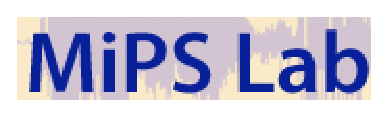
\includegraphics[width=1.75cm]{mips}
%
\epsfig{file=iitk_logo.eps,width=1.5cm}
%\end{center}
%\end{figure}
\begin{figure}[ht]
\begin{center}

\includegraphics[width=1.75cm]{iitk_logo-eps-converted-to.pdf}
%
\epsfig{file=iitk_logo.eps,width=1.5in}
\end{center}
\end{figure}
%\begin{figure}
%\begin{center}
%\hspace{-.0cm}
%\vspace{2cm}\includegraphics[width=1.25cm]{mips-eps-converted-to.pdf}
%\end{center}
%\end{figure}
\end{frame}

%%%%%%%%%%%%%%%%%%%%%%%%%%%%
\begin{frame}{Outline}
\begin{enumerate}
	\vfill\item Multi-Label Document Categorization
	\vfill\item Related Work
	\begin{itemize}
	  \vfill\item Text Representations
	  \vfill\item Learning Algorithms
	\end{itemize}  
	\vfill\item Distributed Word Representations
	\vfill\item Learning Distributed Document Representations
	\vfill\item Document Categorization Algorithm
	\vfill\item Results
	\vfill\item Conclusion and Future Work
\end{enumerate}
\end{frame}

%%%%%%%%%%%%%%%%%%%%%%%%%%%%

\begin{frame}{Introduction to Multi-Label Document Categorization}
\vfill\onslide<1->{\begin{center}
	\emph{Document Categorization} is the task of assigning categories to documents \end{center}
}
\vfill
\onslide<2->{
	\textbf{Why need Multi-Label Document Categorization?}
}
\begin{itemize}
	\vfill\item<3-> Text Documents usually belong to more than one conceptual class. \\For E.g. an article on Music Piracy 
	\vfill\item<4-> Wide range real-world applications :
	\begin{itemize} 
	  \vfill\item<4-> Web-page tagging
	  \vfill\item<4-> Medical Patient Record Management
	  \vfill\item<4-> Wikipedia Article Management
	  \vfill\item<4-> Document Recommendation etc.
	\end{itemize} 
	%\vfill\item<5-> Multi-label classification belongs to a general class of supervised learning algorithms where : 
	% \begin{itemize}
	%   \vfill\item<6-> Training instances in the form of document-category pairs are used to learn a classifier $\mathcal{H}$ 
	%   \vfill\item<7-> Learned classifier $\mathcal{H}$ is used to assign categories to new test documents
	% \end{itemize}
\end{itemize}
\vfill
\end{frame}

%%%%%%%%%%%%%%%%%%%%%%%%%%%%

\begin{frame}{Introduction to Multi-Label Document Categorization}
\vfill\onslide<1->{ Multi-label classification belongs to a general class of \emph{supervised learning} algorithms where, given,  } \\
\begin{itemize} 
	\vfill\item<1-> A set of documents $D = \{d_{1}, \ldots, d_{|D|}\}$
	\vfill\item<1-> A set of categories $C = \{c_{1}, \ldots, c_{|C|}\}$
	\vfill\item<1-> Training data for $n$ {\small ($n < |D|$)} documents, $\traindata = \{l_{d_{1}}, \ldots, l_{d_{n}}\}$ 
%\onslide<4->{   \\ Each label vector $l_{d_{i}} \in \{0,1\}^{|C|}$ denotes relevance of categories to the document $d_{i}$ }
\end{itemize} 
\vfill
\onslide<1->{
	Example :
	\begin{table}[h!]
	\tabcolsep=0.1cm
	\tiny
	\begin{center}
	\begin{tabular}{c@{\hskip5mm} c c c c c c}
	\toprule
	\textbf{Documents}	&	\textbf{Sports} & \textbf{Music} & \textbf{Arts} & \textbf{Technology}  & \textbf{Literature} & \textbf{Politics}\\
	\cmidrule{1-1}
	\cmidrule{2-7}
	$d_{1}$ & 0 & 0 & 1 & 0 & 1 & 0\\
	$d_{2}$ & 0 & 1 & 1 & 0 & 0 & 1\\
	$d_{3}$ & 1 & 0 & 0 & 1 & 0 & 1\\
	$d_{4}$ & x & x & x & x & x & x\\
	$d_{5}$ & x & x & x & x & x & x\\
	\bottomrule         
	\end{tabular}
	\end{center}
	\end{table}
}
\vfill
\onslide<2->{
Using $\traindata$, $D$ and $C$ the learning algorithm learns a multi-label classifier $\mathcal{H}$ to estimate category label vectors, $l_{d_{j}}$ {\small $(j>n)$} for the test documents. 
}
\vfill
\end{frame}

%%%%%%%%%%%%%%%%%%%%%%%%%%%%

\begin{frame}{Introduction to Multi-Label Document Categorization}
\vfill\onslide<1->{ Document Categorization task has the following two components : }
\begin{enumerate}
	\vfill\item<2-> \emph{Learning Document Representations} %: Representing text documents using numerical vectors that are inputs to the multi-label classifier $\mathcal{H}$
	\begin{itemize}
	 	\vfill\item<2-> Each document $d_{i} \in D$ is represented using a vector $v_{d_{i}} \in \mathbb{R}^{k}$
	 	\vfill\item<2-> Embedding documents in a $k$-dimensional space is called the \emph{Vector Space Model}
	 	\vfill\item<2-> The set $D$ can be represented by a matrix $\matD \in \mathbb{R}^{k \times |D|}$
	 	\vfill\item<2->	Vectors ($v_{d_{i}}$) should encode the semantic content of the documents 
	\end{itemize}

	\vfill\item<3-> \emph{Learning Algorithm}
	\begin{itemize}
	 	\vfill\item<3-> Algorithm to learn the multi-label classifier $\mathcal{H}$
	 \end{itemize}		
\end{enumerate}\vfill 
\end{frame}

%%%%%%%%%%%%%%%%%%%%%%%%%%%%

\begin{frame}{Background on Learning Algorithms}
\vfill
%\onslide<1->{ Learning algorithms can be classified into two classes :  }
\begin{enumerate}
	\vfill\item<2-> \emph{Learning Multiple Binary Classifiers} \\
	\onslide<2->{ {\footnotesize	Algorithms that treat each category assignment independently and learn multiple binary classifiers, one for each category, to make the category assignments} 	} 
	\begin{itemize}
		\vfill\item<3-> Logistic Regression
		\vfill\item<3-> Support Vector Machines (SVM)
		\vfill\item<3-> Neural Networks, E.g. CLASSI, NNet.PARC
		\vfill\item<3-> Naive Bayes
	\end{itemize}

	\vfill\item<4-> \emph{Learning Single Joint Classifier} \\
	\onslide<4->{ {\footnotesize	Algorithms that jointly assign all the categories to a document $d_{i}$, i.e. estimate the complete label vector $l_{d_{i}}$ using a single classifier} 	}
	\begin{itemize}
		\vfill\item<5-> k-Nearest Neighbor (k-NN)
		\vfill\item<5-> Linear Least Square Fit
		\vfill\item<5-> Decision Trees
		\vfill\item<5-> Generative Probabilistic Models
	\end{itemize}
\end{enumerate}
%\onslide<14->{ Learning a single joint classifier is usually better as it is able to exploit the category correlations }
\vfill
\end{frame}

%%%%%%%%%%%%%%%%%%%%%%%%%%%%%%

\begin{frame}{Background on Text Representation}
\vfill
\onslide<1->{
\textbf{Bag of Words Model} }
%Most common method to learn vector representations for a set of documents is the \emph{Bag of Words (BOW)} model 	}
\begin{itemize}
	\vfill\item<1-> Document $d_{i}$ represented by $v_{d_{i}} \in \mathbb{R}^{|V|}$
	\vfill\item<1-> Each element in $v_{d_{i}}$ denotes presence/absence of each word
	\vfill\item<1-> Weighing techniques employed to give importance to important terms
	\begin{itemize}
		\vfill\item<1-> Term Frequency (\emph{tf} )
		\vfill\item<1-> Inverse Document Frequency (\emph{idf} )
		\vfill\item<1-> Term Frequency - Inverse Document Frequency (\emph{tf-idf} ) : \emph{tf} $\times$\emph{idf}
	\end{itemize}
\end{itemize}
\vfill
\onslide<2->{
\textbf{Drawbacks of the Bag-of-Words model} }
\begin{itemize}
	\vfill\item<2-> High-dimensionality
	\vfill\item<2-> Sparsity
	\vfill\item<2-> Inability to encode word contexts
	\vfill\item<2-> Ignores word order
	\vfill\item<2-> Lack of similarity measures
\end{itemize}
\vfill
% \todo{feature selection. Word Embeddings. Our document embedding. Our docu cate. Datasets. Results End}
% \vfill
\end{frame}

%%%%%%%%%%%%%%%%%%%%%%%%%%%%%%

\begin{frame}{\large Background on Feature Selection / Dimensionality Reduction}
\vfill
\onslide<1-> {
Techniques to deal with sparsity and high-dimensionality in BOW }
\begin{itemize}
	\vfill\item<2-> Information Gain \\
	\onslide<2->{ { \scriptsize
	\begin{equation}
	G(t) = -\sum_{i=1}^{|C|} P(c_{i})\log P(c_{i}) + P(t)\sum_{i=1}^{|C|} P(c_{i}|t)\log P(c_{i}|t) + P(\sim t)\sum_{i=1}^{|C|} P(c_{i}|\sim t)\log P(c_{i}|\sim t)
	\end{equation}
	} }
	\vfill\item<3-> Mutual Information \\
	\onslide<3->{ { \scriptsize
	\begin{equation}
	I(t,c) = \log \frac{P(t \wedge c)}{P(t) \times P(c)} \text{,}\qquad I_{avg}(t) = \sum_{i=1}^{|C|} P(c_{i})I(t,c_{i})
	\end{equation}
	} }
	\vfill\item<4-> Latent Semantic Indexing (LSI) \\
					\scriptsize	\begin{equation}
						X = T S D^{T}
					\end{equation}
					$X$ is the Term-Document Matrix
\end{itemize}
\vfill
\end{frame}

% %%%%%%%%%%%%%%%%%%%%%%%%%%%%%%

\begin{frame}{Distributed Word Representations}
%\vfill
\onslide<1->{
Representation of each word $w_{i}$ using vector $v_{w_{i}} \in \mathbb{R}^{k}$ ($k \in [50, 300]$) } \\ \vspace{0.5cm}
\onslide<2->{
\textbf{ Need for Distributed Word Representations} } 
\begin{itemize}
	\vfill\item<3-> Curse of Dimensionality
	\begin{itemize}
		\vfill\item<3-> One-hot representations grow with the size of vocabulary
		\vfill\item<3-> Parameters in language modeling grow exponentially with the size of vocabulary
	\end{itemize}
	\vfill\item<4-> No Word Similarity Measure
	\begin{itemize}
		\vfill\item<4-> One-hot representations are orthogonal representations
		\vfill\item<4-> Cannot capture semantic similarity between words
	\end{itemize}
\end{itemize}
\vfill
\end{frame}

%%%%%%%%%%%%%%%%%%%%%%%%%%%%%%
\begin{frame}{Neural Probabilistic Language Model}
\vfill
\onslide<1->{
\citet{bengio2003neural} developed \emph{Neural Probabilistic Language Model (NPLM)} to learn}%learn distributed word vectors and a probability function that uses these vectors to learn a statistical model of language	}
\begin{enumerate}
\vfill\item<1-> Distributed word vectors
\vfill\item<1-> Probability function to learn a statistical model of language 
\end{enumerate}

\begin{columns}[T]
 \begin{column}{.5\textwidth}
 	\centering
 	\onslide<2->{
 	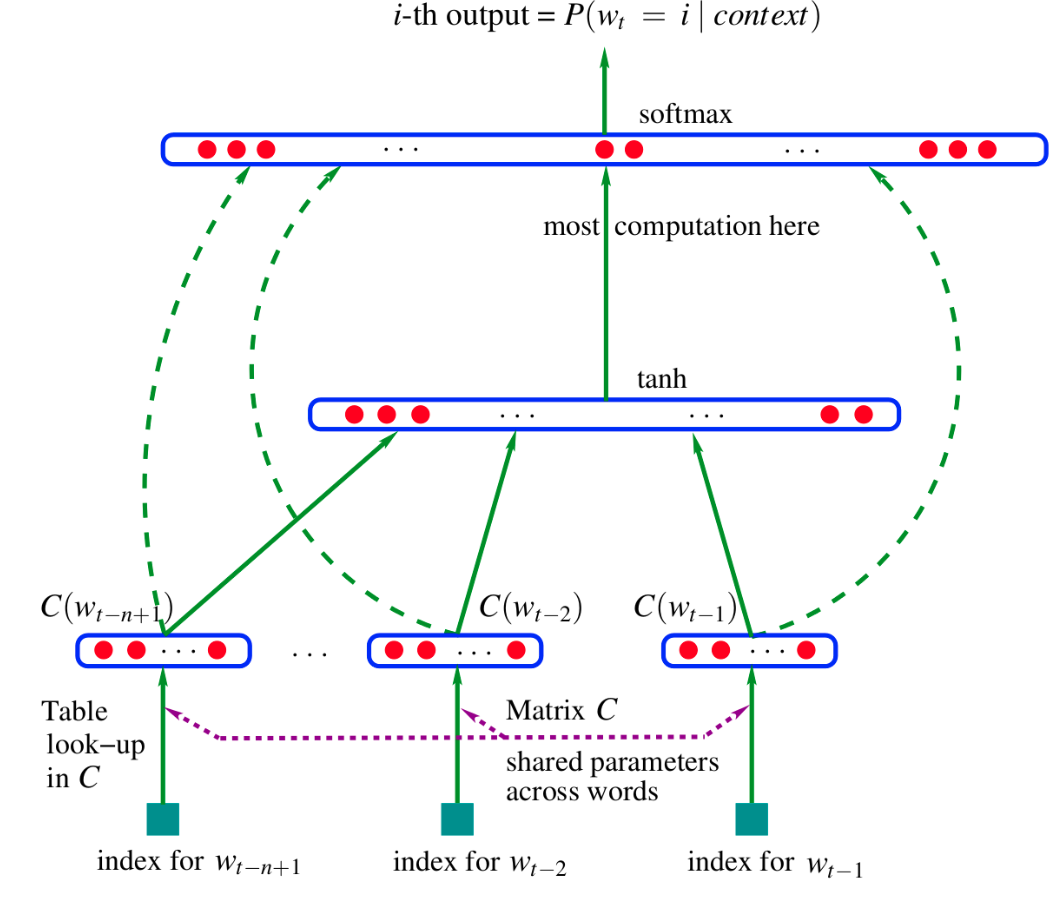
\includegraphics[scale=0.15]{../figs/bengio_nn.png} }

 \end{column}

 \begin{column}{.5\textwidth}
 	\centering
 	{\footnotesize
 	\vfill \onslide<3->{
 	\begin{equation}
    P(w_{t} | w_{1}^{t-1}) \approx P(w_{t} | w_{t-n+1}^{t-1})
    \end{equation} }
    \vfill \onslide<4->{
    \begin{equation}
	y = b + U tanh(d + Hx) \text{,} \quad y \in \mathbb{R}^{|V|}
	\end{equation} }
	\vfill \onslide<5->{
	\begin{equation}
	P(w_{t} | w_{t-1}, \ldots, w_{t-n+1}) = \frac{e^{y_{w_t}}}{\sum_{i}e^{y_{i}}}
	\end{equation} }
	}
 \end{column}
\end{columns}

\vfill
\end{frame}

%%%%%%%%%%%%%%%%%%%%%%%%%%%%%%

\begin{frame}{Log-Linear Models}
\vfill
\onslide<1->{
Proposed by \citet{mikolov2013efficient} to predict words in the context using word vectors}
% \begin{itemize}
% \vfill\item<2-> do not build a language model hence also consider future words in contexts
% \vfill\item<3-> show that the word vectors capture the semantic similarity between words
% \end{itemize}
\vfill
\begin{enumerate}
	\vfill\item<2-> Continuous Bag-of-Words Model 
	\begin{columns}[T]

	 \begin{column}{.5\textwidth}
	 	\centering
	 	\onslide<2->{
	 	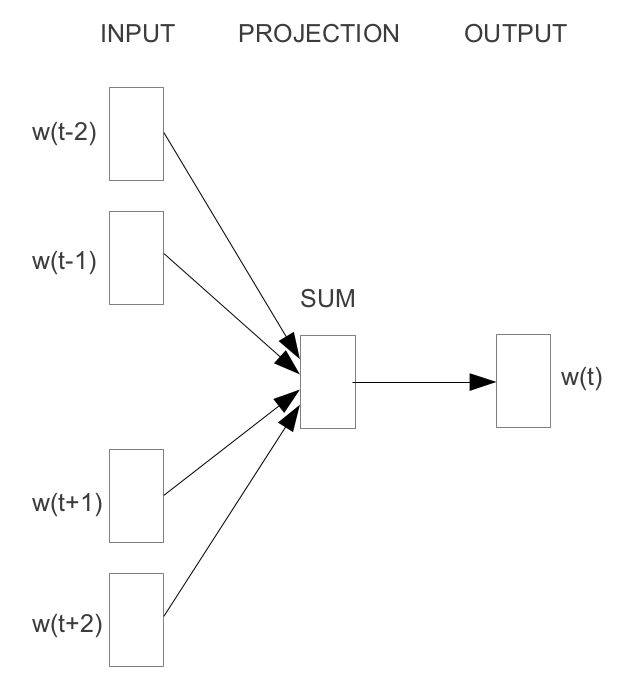
\includegraphics[scale=0.12]{../figs/mikolov_cbow.png} }
	 \end{column}
	 \begin{column}{.5\textwidth}
	 	\centering
	 	{\footnotesize
	 	\onslide<3->{
	 	\begin{equation}
	    h = w_{t-k} + \ldots + w_{t-1} + w_{t+1} + \dots + w_{t+k}
	    \end{equation} }
	    \onslide<4->{
	    \begin{equation}
		y = b + Uh \text{,} \quad y \in \mathbb{R}^{|V|}
		\end{equation} }
		\onslide<5->{
		\begin{equation}
		P(w_{t}|w_{t-k}, \ldots, w_{t+k}) = \frac{e^{y_{w_t}}}{\sum_{i} e^{y_{i}}}
		\end{equation} }
		}
	 \end{column}
	\end{columns}

	\vfill\item<6-> Skip-Gram Model
	\begin{columns}[T]

	 \begin{column}{.5\textwidth}
	 	\centering
	 	\onslide<6->{
	 	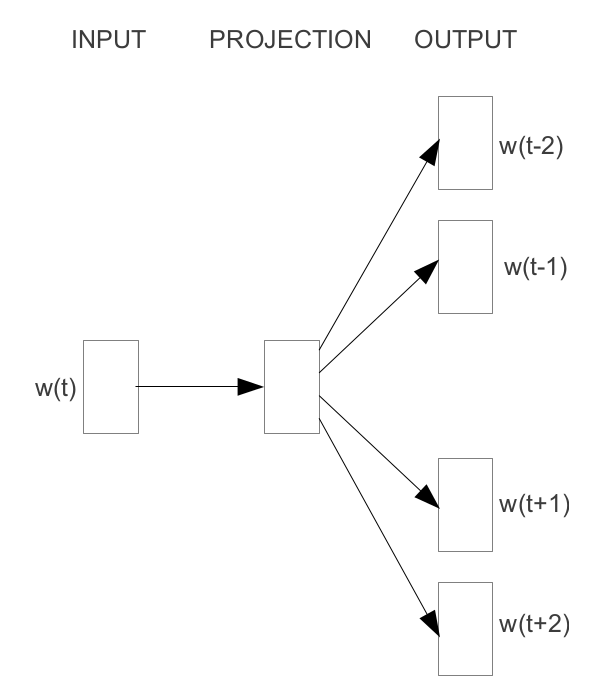
\includegraphics[scale=0.12]{../figs/mikolov_skip.png} }
	 \end{column}
	 \begin{column}{.5\textwidth}
	 	\centering
	 	\vfill
	 	{\footnotesize
	 	\onslide<7->{
	 	\begin{equation}
	    P(w_{t+j}|w_{t}) = \frac{e^{(v_{w_{t}} \cdot v_{w_{t+j}} )} }{\sum_{i} e^{(v_{w_{t}} \cdot v_{w_{i}})} }
	    \end{equation} }
	    }
	 \end{column}
	\end{columns}
\end{enumerate}

\vfill
\end{frame}

%%%%%%%%%%%%%%%%%%%

\begin{frame}{Distributed Document Representations}
\vfill \onslide<1->{
\textbf{Motivation for learning distributed document representations} }
\begin{enumerate}
	\vfill\item<2-> Lack of semantic similarity measures. Therefore, cannot handle synonyms
	\vfill\item<3-> Drawbacks in BOW like sparsity, high-dimensionality, inability to encode context information and consider word ordering
	\vfill\item<4-> Compositionality of word vectors beyond weighted average \cite{mitchell2010composition, zanzotto2010estimating, yessenalina2011compositional, grefenstette2013multi, mikolov2013distributed} 
	\vfill\item<5-> Recursive Tensor Neural Network (RTNN) \cite{socher2013recursive} for learning sentence representations using the syntactic dependency has issues
	\begin{itemize}
		\vfill\item<5-> Parsing, a computationally expensive step required for each sentence
		\vfill\item<5-> Composing sentence vectors to represent documents is not straight-forward
	\end{itemize}
\end{enumerate}
\end{frame}

% %%%%%%%%%%%%%%%%%%%%%%%%%%%%%%%%%%%%%%%%%%


\begin{frame}{Our Model for Learning Document Representations}
\vfill \onslide<1->{
\emph{Inspired by the log-linear models to learn word vectors, we present model, to learn universal distributed representations for documents and words } 
% \begin{quote}
% To learn universal distributed representations for documents and words
% \end{quote}
}
\vfill \onslide<2->{
\textbf{Hypothesis } 
\begin{quote}
Document Representations that encode semantic content of the document should be able to predict words in the document
\end{quote}}

\vfill \onslide<3->{
Our model, }
\begin{enumerate}
	\vfill\item<3-> Learns distributed representations for document (and words) that encode the different semantic content in the documents
	\vfill\item<3-> Embeds documents and words in the same $k$-dimensional space such that semantically similar entities have similar vector representations
\end{enumerate}

\end{frame}
% %%%%%%%%%%%%%%%%%%%%%%%%%%%%%%%%%%%%%%%%%%

\begin{frame}{Our Model for Learning Document Representations}
% \vfill\onslide<1->{
% We present an unsupervised neural network model that, }
% \begin{enumerate}
% 	\vfill\item<1-> Represents each document and word with a $k$-dimensional vector
% 	\vfill\item<2-> Estimates the probability of predicting the middle word in a given word sequence
% 	\vfill\item<3-> Learns document and word vectors and the parameters of the probability function using training corpus
% \end{enumerate}	
\vfill\onslide<1->{
We present an unsupervised neural network model that, }
\begin{enumerate}
	\vfill\item<2-> Represents each document $d_{i} \in D$ by a vector $\vecdi{i} \in \mathbb{R}^{k}$\\
	%Vectors are stored as columns of the matrix $\matD = \left[\vecdi{1}, \ldots, \vecdi{|\setD|}\right] \in \mathbb{R}^{k \times |\setD|}$
	\vfill\item<3-> Each word $w_{i} \in W$, is represented by a vector $\vecwi{i} \in \mathbb{R}^{k}$
	%Vectors are stored as columns of the matrix $\matW = \left[\vecwi{1}, \ldots, \vecwi{|\setW|}\right] \in \mathbb{R}^{k \times |\setW|}$
	\vfill\item<4-> Given a sequence of words, $(w_{t-c}, \ldots, w_{t+c})$ in document $d_{i}$, estimates 
	\begin{equation*}
	p(w_{t} | d_{i}, w_{t-c}, \ldots, w_{t-1}, w_{t+1}, \ldots, w_{t+c})
	\end{equation*}
	\vfill\item<5-> Maximizes probability of predicting the middle word correctly to learn vectors
\end{enumerate}	
\end{frame}

% %%%%%%%%%%%%%%%%%%%%%%%%%%%%%%%%%%%%%%%%%%

\begin{frame}{Our Model for Learning Document Representations}
\vfill
\begingroup
\centering
\tikzset{every picture/.style={scale=0.4}}
\usetikzlibrary{calc}

\def\layersep{3.5cm}

\begin{tikzpicture}[shorten >=1pt,->,draw=black!50, node distance=\layersep,transform shape,rotate=90]  %<-- rotate the NN
	
	\newcommand{\inputsep}{2}
	\newcommand{\docnodey}{0}
	\newcommand{\docinputsep}{2.0}
	\newcommand{\docmiddlesep}{3.2}
	\newcommand{\wordneuron}{1.2}
	

	\newcommand{\iy}{\docnodey - \docinputsep}
	\newcommand{\iiy}{\docnodey - \docinputsep - \inputsep}
	\newcommand{\iiiy}{\docnodey - \docinputsep - \inputsep - \inputsep}
	\newcommand{\iiiiy}{\docnodey - \docinputsep - \inputsep - \inputsep - \inputsep}
	\newcommand{\mwy}{\docnodey + \docmiddlesep}
	\newcommand{\edgestyle}{below}

	\newcommand{\word}[1]{\parbox[t][][r]{8mm}{\centering \footnotesize #1}}

    \tikzstyle{every pin edge}=[<-,shorten <=1pt]
    \tikzstyle{neuronrect}=[rectangle,fill=black!25, minimum size=17pt, inner sep=0pt] %
    \tikzstyle{neuroncircle}=[circle,fill=black!25,minimum size=17pt,inner sep=0pt]
    \tikzstyle{vecrect} = [draw,fill=green!50, minimum width=0.2,minimum height=1cm]
    \tikzstyle{docrect} = [draw,fill=purple!50, minimum width=0.2,minimum height=1cm]
    \tikzstyle{hrect} = [draw,fill=blue!50, minimum width=0.2,minimum height=1cm]
    \tikzstyle{input neuron}=[neuronrect, fill=green!50];
    \tikzstyle{doc neuron}=[neuronrect, fill=purple!50];
    \tikzstyle{output neuron}=[neuroncircle, fill=red!50];
    \tikzstyle{hidden neuron}=[neuronrect, fill=blue!50];
    \tikzstyle{annot} = [text width=4em, text centered]
    \tikzset{hoz/.style={rotate=-90}}   %<--- for labels
    % Draw the input layer nodes
    %\foreach \name / \y in {1,...,4}
    % This is the same as writing \foreach \name / \y in {1/1,2/2,3/3,4/4}
        %\node[input neuron, pin=left:\rotatebox{-90}{\parbox[t][][r]{8mm}{\centering $w_{t-j}$}}] (I-\name) at (0,-\y) {};

    %Centre Word    
    \node[pin=left:\rotatebox{-90}{\word{Metallica}}] (I-1) at (-\wordneuron,\mwy) {};
	%\node[input neuron, pin=left:\rotatebox{-90}{\parbox[t][][r]{8mm}{\centering $w_{t}$}}] (W-0) at (0,\mwy) {};    
	\node[vecrect, pin=left:\rotatebox{-90}{\parbox[t][][r]{8mm}{\centering $w_{t}$}}] (W-0) at (0,\mwy) {};    

	%\node (rect) at (4,2) [draw,thick,fill=green!50, minimum width=0.2,minimum height=2cm, pin=left:\rotatebox{-90}{\word{Rolling\\Stones}}] {};
	
	%Doc 
	\node[pin=left:\rotatebox{-90}{\word{Rolling\newline Stones}}] (I-1) at (-\wordneuron,\docnodey) {};
    %\node[doc neuron, pin=left:\rotatebox{-90}{\parbox[t][][r]{8mm}{\centering $d_{i}$}}] (D-0) at (0,\docnodey) {};    
    \node[docrect, pin=left:\rotatebox{-90}{\parbox[t][][r]{8mm}{\centering $d_{i}$}}] (D-0) at (0,\docnodey) {};    

    \node[pin=left:\rotatebox{-90}{\word{metal}}] (I-1) at (-\wordneuron,\iy) {};
    %\node[input neuron, pin=left:\rotatebox{-90}{\parbox[t][][r]{8mm}{\centering $w_{t-2}$}}] (W-1) at (0,\iy) {};
    \node[vecrect, pin=left:\rotatebox{-90}{\parbox[t][][r]{8mm}{\centering $w_{t-2}$}}] (W-1) at (0,\iy) {};

    \node[pin=left:\rotatebox{-90}{\word{band}}] (I-1) at (-\wordneuron,\iiy) {};
    %\node[input neuron, pin=left:\rotatebox{-90}{\parbox[t][][r]{8mm}{\centering $w_{t-1}$}}] (W-2) at (0,\iiy) {};
    \node[vecrect, pin=left:\rotatebox{-90}{\parbox[t][][r]{8mm}{\centering $w_{t-1}$}}] (W-2) at (0,\iiy) {};
    
    \node[pin=left:\rotatebox{-90}{\word{plays}}] (I-1) at (-\wordneuron,\iiiy) {};
    %\node[input neuron, pin=left:\rotatebox{-90}{\parbox[t][][r]{8mm}{\centering $w_{t+1}$}}] (W-3) at (0,\iiiy) {};
    \node[vecrect, pin=left:\rotatebox{-90}{\parbox[t][][r]{8mm}{\centering $w_{t+1}$}}] (W-3) at (0,\iiiy) {};

    \node[pin=left:\rotatebox{-90}{\word{today}}] (I-1) at (-\wordneuron,\iiiiy) {};
    \node[vecrect, pin=left:\rotatebox{-90}{\parbox[t][][r]{8mm}{\centering $w_{t+2}$}}] (W-4) at (0,\iiiiy) {};    
    %\node[input neuron, pin=left:\rotatebox{-90}{\parbox[t][][r]{8mm}{\centering $w_{t+2}$}}] (W-4) at (0,\iiiiy) {};    

    % Draw the hidden layer nodes
    % \foreach \name / \y in {1,...,5}
        \path[yshift=0.5cm]
        %node[hidden neuron] (P-1) at (\layersep,\iy - 1) [label=below:\rotatebox{-90}{\parbox[t][][r]{2mm}{\centering \footnotesize $h_{c}$}}] {};
        node[hrect] (P-1) at (\layersep,\iy - 1) [label=below:\rotatebox{-90}{\parbox[t][][r]{2mm}{\centering \footnotesize $h_{c}$}}] {};

    % Draw the output layer node
    \node[output neuron, pin={[pin edge={->}]right:\rotatebox{-90}{$p(w_{t}|d_{i}, w_{t-2}, w_{t-1}, w_{t+1}, w_{t+2})$}}] (O) at (\layersep + \layersep,0) {};
    %\node[output neuron,pin={[pin edge={->}]right:\rotatebox{-90}{$p(w_{t}|d_{i}, w_{t-2}, \ldots, w_{t+2})$}}, right of=H-1] (O) {};

    % Connect word vectors to projection later
     \path (W-1) edge node[\edgestyle] {\rotatebox{-90}{\tiny $\wgt{t-2}$}} (P-1);
     \path (W-2) edge node[\edgestyle] {\rotatebox{-90}{\tiny $\wgt{t-1}$}} (P-1);
     \path (W-3) edge node[\edgestyle] {\rotatebox{-90}{\tiny $\wgt{t+1}$}} (P-1);
     \path (W-4) edge node[\edgestyle] {\rotatebox{-90}{\tiny $\wgt{t+2}$}} (P-1);   

    %Connect Middle Word to Output Node
	\path [->,font=\scriptsize] (W-0) edge (O);            

	%Connect Doc Embedding to Projection Layer
	\path (D-0) edge (P-1);            

    %Connect Projection Layer to Output
    \path (P-1) edge (O);

    % Annotate the layers
    \node[annot,above of=P-1, node distance=7.1cm,hoz] (hl) {\footnotesize Projection layer};
    \node[annot,left of=hl,hoz] {\footnotesize Input layer};
    \node[annot,right of=hl,hoz] {\footnotesize Output layer};
\end{tikzpicture}

% \begin{tikzpicture}[scale=1.0, transform shape]
% % Macros
% % relative positioning
% \newcommand{\at}[3]{
%   \begin{scope}[shift={(#1,#2)}]
%     #3
%   \end{scope} 
% }

% % Embeddings
% \newcommand{\embcolor}{PineGreen}
% \newcommand{\ye}{1}
% \newcommand{\he}{1.5}
% \newcommand{\we}{1}
% \newcommand{\gape}{1}

% \newcommand{\xc}{0.5}
% \newcommand{\xa}{\xc+\we+\gape}
% \newcommand{\xb}{\xa+\we+\gape}
% \newcommand{\xu}{\xb+\we+\gape}
% \newcommand{\xw}{\xu+\we+\gape}

% \draw [thick]
% 	(\xb+\we/2,\ye+\he+0.5) node[above,\embcolor] {Entities, $\mathcal{E}$};
% % Draw curly braces using path decoration
% \draw [\embcolor,decorate,decoration={brace,amplitude=5pt},xshift=-15pt] %,yshift=-9pt] 
% 	(\xc,\ye)  -- (\xc,\ye+\he) node [align=right,left,\embcolor,midway,xshift=-5pt]
% 	{Model Parameters, $\Phi$\\{\small $k$-dimensional entity vectors}};
% % Users
% \draw[<->,\embcolor!50]
% 	(\xu,\ye-0.15) -- (\xu+\we,\ye-0.15) 
% 	node[pos=.5,shape=rectangle,fill=white,draw=none] {\scriptsize $k$};
% \draw[<->,\embcolor!50] 
% 	(\xu+\we+0.3,\ye) -- (\xu+\we+0.3,\ye+\he) 
% 	node[pos=.5,shape=rectangle,fill=white,draw=none] {\scriptsize $|U|$};
% \draw [semithick,fill=gray!10] 
% 	(\xu,\ye) rectangle (\xu+\we,\ye+\he)
% 	(\xu+\we/2.0,\ye+\he/2.0) node[draw=none,shape=circle] (nodeU) {$\Phi_U$}
% 	(\xu+\we/2.0,\ye+\he) node[above] {\scriptsize Users, U};
% % Businesses
% \draw[<->,\embcolor!50]
% 	(\xb,\ye-0.15) -- (\xb+\we,\ye-0.15) 
% 	node[pos=.5,shape=rectangle,fill=white,draw=none] {\scriptsize $k$};
% \draw[<->,\embcolor!50] 
% 	(\xb+\we+0.3,\ye) -- (\xb+\we+0.3,\ye+\he) 
% 	node[pos=.5,shape=rectangle,fill=white,draw=none] {\scriptsize $|B|$};
% \draw [semithick,fill=gray!10] 
% 	(\xb,\ye) rectangle (\xb+\we,\ye+\he)
% 	(\xb+\we/2.0,\ye+\he/2.0) node[draw=none,shape=circle] (nodeB) {$\Phi_B$}
% 	(\xb+\we/2.0,\ye+\he) node[above] {\scriptsize Businesses, B};
% % Categories
% \draw[<->,\embcolor!50]
% 	(\xc,\ye-0.15) -- (\xc+\we,\ye-0.15) 
% 	node[pos=.5,shape=rectangle,fill=white,draw=none] {\scriptsize $k$};
% \draw[<->,\embcolor!50] 
% 	(\xc+\we+0.3,\ye) -- (\xc+\we+0.3,\ye+\he) 
% 	node[pos=.5,shape=rectangle,fill=white,draw=none] {\scriptsize $|C|$};
% \draw [semithick,fill=gray!10] 
% 	(\xc,\ye) rectangle (\xc+\we,\ye+\he)
% 	(\xc+\we/2.0,\ye+\he/2.0) node[draw=none,shape=circle] (nodeC) {$\Phi_C$}
% 	(\xc+\we/2.0,\ye+\he) node[above] {\scriptsize Categories, C};
% % Attributes
% \draw[<->,\embcolor!50]
% 	(\xa,\ye-0.15) -- (\xa+\we,\ye-0.15) 
% 	node[pos=.5,shape=rectangle,fill=white,draw=none] {\scriptsize $k$};
% \draw[<->,\embcolor!50] 
% 	(\xa+\we+0.3,\ye) -- (\xa+\we+0.3,\ye+\he) 
% 	node[pos=.5,shape=rectangle,fill=white,draw=none] {\scriptsize $|A|$};
% \draw [semithick,fill=gray!10] 
% 	(\xa,\ye) rectangle (\xa+\we,\ye+\he)
% 	(\xa+\we/2.0,\ye+\he/2.0) node[draw=none,shape=circle] (nodeA) {$\Phi_A$}
% 	(\xa+\we/2.0,\ye+\he) node[above] {\scriptsize Attributes, A};
% % Words
% \draw[<->,\embcolor!50]
% 	(\xw,\ye-0.15) -- (\xw+\we,\ye-0.15) 
% 	node[pos=.5,shape=rectangle,fill=white,draw=none] {\scriptsize $k$};
% \draw[<->,\embcolor!50] 
% 	(\xw+\we+0.3,\ye) -- (\xw+\we+0.3,\ye+\he) 
% 	node[pos=.5,shape=rectangle,fill=white,draw=none] {\scriptsize $|W|$};
% \draw [semithick,fill=gray!10] 
% 	(\xw,\ye) rectangle (\xw+\we,\ye+\he)
% 	(\xw+\we/2.0,\ye+\he/2.0) node[draw=none,shape=circle] (nodeW) {$\Phi_W$}
% 	(\xw+\we/2.0,\ye+\he) node[above] {\scriptsize Review words, W};

% % Matrices (Relations)
% \newcommand{\relcolor}{RoyalBlue}
% \newcommand{\ym}{-2}
% \newcommand{\hm}{2}
% \newcommand{\wm}{2}
% \newcommand{\gapm}{0.75}
% \newcommand{\gridmcolor}{gray!10}

% \newcommand{\xCB}{-2}
% \newcommand{\xAB}{\xCB+\wm+\gapm}
% \newcommand{\xR}{\xAB+\wm+\gapm}
% \newcommand{\xBW}{\xR+\wm+\gapm}
% \newcommand{\xUW}{\xBW+\wm+\gapm}

% \newcommand{\sparsegrid}{
% 	\draw [step=0.1,thin,\gridmcolor] (0,0) grid (\wm,\hm);
% 	\foreach \i in {0,1,...,75}{
% 		\pgfmathsetmacro{\xcell}{int(rnd*20)*\wm/20}
% 		\pgfmathsetmacro{\ycell}{int(rnd*20)*\wm/20}
% 		\fill[gray!20] (\xcell,\ycell) rectangle (\xcell+0.1,\ycell+0.1);
% 	}
% }

% \draw [thick]
% 	(\xR+\wm/2,\ym-0.5) node[below,\relcolor] {Relations, $\mathcal{R}$};
% % Draw curly braces using path decoration
% \draw [\relcolor,decorate,decoration={brace,amplitude=5pt},xshift=-15pt] %,yshift=-9pt] 
% 	(\xCB,\ym)  -- (\xCB,\ym+\hm) node [align=right,left,\relcolor,midway,xshift=-5pt]
% 	{Partial Observations\\{\small Predict missing data}};

% % CB
% \draw[<->,\relcolor!50]
% 	(\xCB,\ym+\hm+0.15) -- (\xCB+\wm,\ym+\hm+0.15) 
% 	node[pos=.5,shape=rectangle,fill=white,draw=none] {\scriptsize $|C|$};
% \draw[<->,\relcolor!50] 
% 	(\xCB+\wm+0.3,\ym) -- (\xCB+\wm+0.3,\ym+\hm) 
% 	node[pos=.5,shape=rectangle,fill=white,draw=none] {\scriptsize $|B|$};
% \at{\xCB}{\ym}{\sparsegrid}
% \draw [thick] 
% 	(\xCB,\ym) rectangle (\xCB+\wm,\ym+\hm)
% 	(\xCB+\wm/2.0,\ym+\hm/2.0) node[draw=none,shape=circle] (nodeCB) {C}
% 	(\xCB+\wm/2.0,\ym) node[below] {\scriptsize Business Categories};
% % AB
% \draw[<->,\relcolor!50]
% 	(\xAB,\ym+\hm+0.15) -- (\xAB+\wm,\ym+\hm+0.15) 
% 	node[pos=.5,shape=rectangle,fill=white,draw=none] {\scriptsize $|A|$};
% \draw[<->,\relcolor!50] 
% 	(\xAB+\wm+0.3,\ym) -- (\xAB+\wm+0.3,\ym+\hm) 
% 	node[pos=.5,shape=rectangle,fill=white,draw=none] {\scriptsize $|B|$};
% \at{\xAB}{\ym}{\sparsegrid}
% \draw [thick] 
% 	(\xAB,\ym) rectangle (\xAB+\wm,\ym+\hm)
% 	(\xAB+\wm/2.0,\ym+\hm/2.0) node[draw=none,shape=circle] (nodeAB) {A}
% 	(\xAB+\wm/2.0,\ym) node[below] {\scriptsize Business Attributes};
% % R
% \draw[<->,\relcolor!50]
% 	(\xR,\ym+\hm+0.15) -- (\xR+\wm,\ym+\hm+0.15) 
% 	node[pos=.5,shape=rectangle,fill=white,draw=none] {\scriptsize $|U|$};
% \draw[<->,\relcolor!50] 
% 	(\xR+\wm+0.3,\ym) -- (\xR+\wm+0.3,\ym+\hm) 
% 	node[pos=.5,shape=rectangle,fill=white,draw=none] {\scriptsize $|B|$};
% \at{\xR}{\ym}{\sparsegrid}
% \draw [thick] 
% 	(\xR,\ym) rectangle (\xR+\wm,\ym+\hm)
% 	(\xR+\wm/2.0,\ym+\hm/2.0) node[draw=none,shape=circle] (nodeR) {R}
% 	(\xR+\wm/2.0,\ym) node[below] {\scriptsize User/Business Ratings};
% % BW
% \draw[<->,\relcolor!50]
% 	(\xBW,\ym+\hm+0.15) -- (\xBW+\wm,\ym+\hm+0.15) 
% 	node[pos=.5,shape=rectangle,fill=white,draw=none] {\scriptsize $|W|$};
% \draw[<->,\relcolor!50] 
% 	(\xBW+\wm+0.3,\ym) -- (\xBW+\wm+0.3,\ym+\hm) 
% 	node[pos=.5,shape=rectangle,fill=white,draw=none] {\scriptsize $|B|$};
% \at{\xBW}{\ym}{\sparsegrid}
% \draw [thick] 
% 	(\xBW,\ym) rectangle (\xBW+\wm,\ym+\hm)
% 	(\xBW+\wm/2.0,\ym+\hm/2.0) node[draw=none,shape=circle] (nodeBW) {BW}
% 	(\xBW+\wm/2.0,\ym) node[below] {\scriptsize Reviews for Business};
% % UW
% \draw[<->,\relcolor!50]
% 	(\xUW,\ym+\hm+0.15) -- (\xUW+\wm,\ym+\hm+0.15) 
% 	node[pos=.5,shape=rectangle,fill=white,draw=none] {\scriptsize $|W|$};
% \draw[<->,\relcolor!50] 
% 	(\xUW+\wm+0.3,\ym) -- (\xUW+\wm+0.3,\ym+\hm) 
% 	node[pos=.5,shape=rectangle,fill=white,draw=none] {\scriptsize $|U|$};
% \at{\xUW}{\ym}{\sparsegrid}
% \draw [thick] 
% 	(\xUW,\ym) rectangle (\xUW+\wm,\ym+\hm)
% 	(\xUW+\wm/2.0,\ym+\hm/2.0) node[draw=none,shape=circle] (nodeUW) {UW}
% 	(\xUW+\wm/2.0,\ym) node[below] {\scriptsize Reviews by Users};

% % Edges between embeddings and matrices
% \newcommand{\arrowcolor}{black}
% \draw[\arrowcolor,->] (nodeC) -- (nodeCB);
% \draw[\arrowcolor,->] (nodeB) -- (nodeCB);

% \draw[\arrowcolor,->] (nodeA) -- (nodeAB);
% \draw[\arrowcolor,->] (nodeB) -- (nodeAB);

% \draw[\arrowcolor,->] (nodeU) -- (nodeR);
% \draw[\arrowcolor,->] (nodeB) -- (nodeR);

% \draw[\arrowcolor,->] (nodeW) -- (nodeBW);
% \draw[\arrowcolor,->] (nodeB) -- (nodeBW);

% \draw[\arrowcolor,->] (nodeU) -- (nodeUW);
% \draw[\arrowcolor,->] (nodeW) -- (nodeUW);
% \end{tikzpicture}%
\endgroup
\footnotesize{
	\vfill
	\onslide<2->{
		\textbf{Context Representation} : 
		\begin{equation}
		h_{c} = \vecdi{d_{i}} + \wgt{t-c}\vecwi{w_{t-c}} + \ldots + \wgt{t-1}\vecwi{w_{t-1}} + \wgt{t+1}\vecwi{w_{t+1}} + \ldots + \wgt{t+c}\vecwi{w_{t+c}}
		\end{equation}
		\vfill
	} \onslide<3->{
		\textbf{Probability Estimation} : 
		\begin{equation}
		s_{w_{i}} = \sigma(\vecwi{w_{i}}\cdot h_{c}) \text{,} \quad  \sigma(x) = \frac{1}{1 + e^{-x}}
		\end{equation}
		\begin{equation}
		p(w_{t} | d_{i}, w_{t-c}, \ldots, w_{t-1}, w_{t+1}, \ldots, w_{t+c}) = \frac{e^{s_{w_{t}}}}{\sum_{i \in \setW} e^{s_{w_{i}}}}
		\end{equation}
	}
\vfill
}
\end{frame}

 %%%%%%%%%%%%%%%%%%%%%%%%%%%%%%%%%%%%%%%%%%%%

\begin{frame}{Training Objective}
\vfill
\begin{enumerate}
	\vfill\item<1-> Training data $\traindata$ = $\{d^{(m)}_{i}, w^{(m)}_{t-c}, \ldots, w^{(m)}_{t+c}\}^{m=M}_{m=1}$
	\vfill\item<2-> Learn optimum parameter set $\Theta = (\matD, \matW, \Lambda)$, i.e. document and word vectors and the neural network weights $\Lambda$ 
	\vfill\item<3-> Maximize average log-probability of predicting $w_{t}$ correctly in each sequence in $\traindata$
					\begin{equation}
						\hat{\Theta} =  \argmax_{\Theta}~l(\traindata, \Theta)
					\end{equation}
					\begin{equation}
						l(\traindata, \Theta) = \frac{1}{M}\sum_{m=1}^{M} \log \left[p(w^{(m)}_{t} | d^{(m)}_{i}, w^{(m)}_{t-c}, \ldots, w^{(m)}_{t-1}, w^{(m)}_{t+1}, \ldots, w^{(m)}_{t+c})\right]
					\end{equation}
	\vfill\item<4-> Use Stochastic Gradient Descent (SGD) to update parameters
					\begin{equation}
						\theta^{(x)}_{i} = \theta^{(x-1)}_{i} + \gamma\frac{\partial l(\traindata, \Theta)}{\partial \theta_{i}}
					\end{equation}
\end{enumerate}
	

\end{frame}

 %%%%%%%%%%%%%%%%%%%%%%%%%%%%%%%%%%%%%%%%%%%%

\begin{frame}{Noise Contrastive Estimation}
\vfill
\begin{enumerate}
	\vfill\item<1-> Soft-max computation is expensive, $\mathcal{O}$($\setW$)
	\vfill\item<2-> Speed-ups using \textbf{Hierarchical soft-max} \citep{morin2005hierarchical} and \textbf{Importance sampling} to approximate the likelihood gradient \citep{bengio2003quick, bengio2008adaptive}
	\begin{itemize}
		\vfill\item<2-> Finding well-performing trees in Hierarchical soft-max is not trivial
		\vfill\item<2-> Importance sampling suffers from stability issues
	\end{itemize}
	\vfill\item<3-> \textbf{Noise Contrastive Estimation} (NCE) \citep{gutmann2012noise} fits unnormalized probabilities
	\begin{itemize}
		\vfill\item<3-> Reduces the problem of \emph{probability density estimation} to \emph{probabilistic binary classification}
		\vfill\item<3-> Adaptation to NPLM \citep{mnih2012fast} and learning word embeddings \citep{mnih2013learning} show significant training time speed-ups
	\end{itemize}
\end{enumerate}
\end{frame}

 %%%%%%%%%%%%%%%%%%%%%%%%%%%%%%%%%%%%%%%%%%%%

\begin{frame}{Noise Contrastive Estimation (contd.)}
\vfill
\begin{enumerate}
	\vfill\item<1-> Given a sequence of words $(w_{t-c}, \ldots, w_{t+c})$ in document $d_{i}$
	\begin{itemize}
		\vfill\item<2-> \emph{Earlier objective} : Maximize $p(w_{t} | d_{i}, w_{t-c}, \ldots, w_{t-1}, w_{t+1}, \ldots, w_{t+c})$	
		\vfill\item<3-> \emph{New objective}	 : Build binary classifier to distinguish between correct middle word $w_{t}$ and random corrupt word 	
	\end{itemize}
\end{enumerate}
\vfill \onslide<4->{
\textbf{For NCE Binary Classification Objective : }
}
\begin{enumerate}
	\vfill\item<5-> New labeled training data : $\traindata$ = $\{d^{(m)}_{i}, w^{(m)}_{t-c}, \ldots, w^{(m)}_{t+c}, Y^{(m)}=1\}^{m=M}_{m=1}$
	\vfill\item<6-> For every positive training sequence, $n$ negative training sequences introduced where,
	\begin{itemize}
		\vfill\item<6-> The observed middle word $w_{t}$ is replaced by a corrupt word $w_{x}$ drawn from a noise distribution $P_{n}(w)$
		\vfill\item<6-> E.g. $\{d_{i}, w_{t-c}, \ldots, w_{t-1}, w_{x}, w_{t+1}, \ldots, w_{t+c}, Y=0\}$ %The label for the negative sequence is $Y = 0$
	\end{itemize}
	\vfill\item<7-> Complete training data : $\traindata$ = $\{d^{(m)}_{i}, w^{(m)}_{t-c}, \ldots, w^{(m)}_{t+c}, Y^{(m)}\}^{m=M+nM}_{m=1}$
\end{enumerate}

\end{frame}

 %%%%%%%%%%%%%%%%%%%%%%%%%%%%%%%%%%%%%%%%%%%%

\begin{frame}{Noise Contrastive Estimation (contd.)}
\vfill
\vfill\onslide<1-> {
 	Given a sequence of words $(w_{t-c}, \ldots, w_{t+c})$ in document $d_{i}$, our new objective is to predict whether the sequence is legitimate
}
\begin{itemize}
	\vfill\item<2-> We build a probabilistic binary classifier to predict the label $Y$
	\vfill\onslide<2-> { \begin{equation}
	P(Y=1|d_{i}, w_{t-c}, \ldots, w_{t+c}, \Theta) = \sigma(\vecwi{w_{t}} \cdot h_{c})
	\end{equation} }
	\vfill\onslide<3-> { \begin{equation}
	P(Y=0|d_{i}, w_{t-c}, \ldots, w_{t+c}, \Theta) = 1 - \sigma(\vecwi{w_{t}} \cdot h_{c})
	\end{equation} }
	\vfill\onslide<4-> { \begin{equation}
	P(Y|d_{i}, w_{t-c}, \ldots, w_{t+c}, \Theta) = [\sigma(\vecwi{w_{t}} \cdot h_{c})]^{Y}[1 - \sigma(\vecwi{w_{t}} \cdot h_{c})]^{1-Y}
	\end{equation} }
\end{itemize}

\end{frame}

%%%%%%%%%%%%%%%%%%%%%%%%%%%%%%%%%%%%%%%%%%%%

\begin{frame}{Learning Objective with NCE}
\vfill
\vfill\onslide<1-> {
 	Given the training data $\traindata$ = $\{d^{(m)}_{i}, w^{(m)}_{t-c}, \ldots, w^{(m)}_{t+c}, Y^{(m)}\}^{m=M+nM}_{m=1}$, we maximize the log-likelihood of observing it
}
\vfill\onslide<2-> { \begin{equation}
 	\hat{\Theta} =  \argmax_{\Theta}~l(\traindata, \Theta)
 	\end{equation}
 	\begin{equation}
 	l(\traindata, \Theta) = \sum_{m=1}^{M + nM} \log P_{\Theta}(Y_{m} = Y^{(m)})
 	\end{equation}
 	\blfootnote{$P_{\Theta}(Y_{m})$ is a shorthand notation for $P(Y_{m}|d^{(m)}_{i}, w^{(m)}_{t-c}, \ldots, w^{(m)}_{t+c}, \Theta)$ }
 	\blfootnote{$Y_{m}$ is the predicted label}
}
\vfill\onslide<3-> {
The logarithm of the probability estimate is given by,
\footnotesize{
\begin{equation}
\log P_{\Theta}(Y_{m} = Y^{(m)}) = Y^{(m)}\log \sigma(\vecwi{w^{(m)}_{t}} \cdot h^{(m)}_{c}) + (1 - Y^{(m)})\log (1 - \sigma(\vecwi{w^{(m)}_{t}} \cdot h^{(m)}_{c}))
\end{equation} } }

\end{frame}

%%%%%%%%%%%%%%%%%%%%%%%%%%%%%%%%%%%%%%%%%%%%

\begin{frame}{Parameter Estimation}

\vfill\onslide<1-> {
 	We use SGD to learn parameters i.e. document and word vectors and the neural network weights
 	\begin{equation}
		\theta^{(x)}_{i} = \theta^{(x-1)}_{i} + \gamma\frac{\partial l(\traindata, \Theta)}{\partial \theta_{i}}
	\end{equation}
}
\vfill\onslide<2-> { Gradient of $\log P_{\Theta}(Y_{m} = Y^{(m)})$ with respect to parameter $\theta$, }
\vfill\onslide<3-> { \scriptsize{	\begin{equation}
		\frac{\partial \log P_{\Theta}(Y_{m}=Y^{(m)})} {\partial \theta} = \left[ Y^{(m)}\frac{1}{\sigma(d^{(m)})} - (1-Y^{(m)})\frac{1}{(1 - \sigma(d^{(m)}))}\right] \frac{\partial \sigma(d^{(m)})}{\partial \theta} 
\end{equation} } }
\vfill\onslide<4-> { \scriptsize{	\begin{equation}
		\frac{\partial \log P_{\Theta}(Y_{m}=Y^{(m)})} {\partial \theta} = \left[ Y^{(m)}\frac{1}{ \sigma(d^{(m)})} - (1 - Y^{(m)})\frac{1}{(1 - \sigma(d^{(m)}))}\right]
		\left[\sigma(d^{(m)})(1-\sigma(d^{(m)}))\right]\frac{\partial d^{(m)}}{\partial \theta}
\end{equation} } }
\vfill\onslide<5-> { \scriptsize{	\begin{equation}
		\frac{\partial \log P_{\Theta}(Y_{m}=Y^{(m)})} {\partial \theta} = \left[ Y^{(m)} - \sigma(d^{(m)})\right] \frac{\partial d^{(m)}}{\partial \theta}
\end{equation} } }
\vfill\onslide<6-> { \scriptsize{	\begin{equation}
		\frac{\partial \log P_{\Theta}(Y_{m}=Y^{(m)})} {\partial \theta} = \left[ Y^{(m)} - \sigma(\vecwi{w^{(m)}_{t}} \cdot h^{(m)}_{c})\right] \frac{\partial (\vecwi{w^{(m)}_{t}} \cdot h^{(m)}_{c})}{\partial \theta}
\end{equation} } }

\blfootnote{\tiny{$d= \mathrm{v}^{W}_{w_{t}} \cdot h_{c}$, is the pre-sigmoid activation } }

\end{frame}

%%%%%%%%%%%%%%%%%%%%%%%%%%%%%%%%%%%%%%%%%%%%

% \begin{frame}{Parameter Estimation}

% \vfill\onslide<1-> { Gradient of the likelihood w.r.t. various parameters, }

% \begin{enumerate}
% 	\vfill\item<2-> Document Vector : 
% 		\scriptsize{ \begin{equation}
% 				\frac{\partial \log P_{\Theta}(Y_{m}=Y^{(m)})} {\partial \vecdi{d^{(m)}_{i}}} = \left[ Y^{(m)} - \sigma(\vecwi{w^{(m)}_{t}} \cdot h^{(m)}_{c})\right] \vecwi{w^{(m)}_{t}}
% 		\end{equation} }
% 	\vfill\item<3-> Middle Word Vector : 	
% 		\scriptsize{ \begin{equation}
% 			\frac{\partial \log P_{\Theta}(Y_{m}=Y^{(m)})} {\partial \vecwi{w^{(m)}_{t}}} = \left[ Y^{(m)} - \sigma(\vecwi{w^{(m)}_{t}} \cdot h^{(m)}_{c})\right] h^{(m)}_{c}
% 		\end{equation} }
% 	\vfill\item<4-> Context Word Vectors : 		
% 		\scriptsize{	\begin{equation}
% 			\frac{\partial \log P_{\Theta}(Y_{m}=Y^{(m)})} {\partial \vecwi{w^{(m)}_{t+j}}} = \left[ Y^{(m)} - \sigma(\vecwi{w^{(m)}_{t}} \cdot h^{(m)}_{c})\right] \wgt{t+j} \vecwi{w^{(m)}_{t}}
% 		\end{equation} }
% 	\vfill\item<5-> Neural Network Weights : 		
% 		\scriptsize{	\begin{equation}
% 			\frac{\partial \log P_{\Theta}(Y_{m}=Y^{(m)})} {\partial \wgt{t+j}} = \left[ Y^{(m)} - \sigma(\vecwi{w^{(m)}_{t}} \cdot h^{(m)}_{c})\right] (\vecwi{w^{(m)}_{t}} \cdot \vecwi{w^{(m)}_{t+j}})
% 		\end{equation} }
% \end{enumerate}
% \end{frame}

%%%%%%%%%%%%%%%%%%%%%%%%%%%%%%%%%%%%%%%%%%%%

\begin{frame}{Update rule for Parameters}

\begin{enumerate}
	\vfill\item<1-> Document Vector : 
		\scriptsize{ \begin{equation}
				(\vecdi{d^{(m)}_{i}})^{(i+1)} = (\vecdi{d^{(m)}_{i}})^{(i)} + \gamma \left[ (Y^{(m)} - \sigma(\vecwi{w^{(m)}_{t}} \cdot h^{(m)}_{c}) )\vecwi{w^{(m)}_{t}} - \beta\vecdi{d^{(m)}_{i}} \right]
		\end{equation} }
	\vfill\item<2-> Middle Word Vector : 	
		\scriptsize{ \begin{equation}
			(\vecwi{w^{(m)}_{t}})^{(i+1)} = (\vecwi{w^{(m)}_{t}})^{(i)} + \gamma \left[ (Y^{(m)} - \sigma(\vecwi{w^{(m)}_{t}} \cdot h^{(m)}_{c})) h^{(m)}_{c} - \beta\vecwi{w^{(m)}_{t}} \right]
		\end{equation} }
	\vfill\item<3-> Context Word Vectors : 		
		\scriptsize{	\begin{equation}
			(\vecwi{w^{(m)}_{t+j}})^{(i+1)} = (\vecwi{w^{(m)}_{t+j}})^{(i)} + \gamma \left[(Y^{(m)} - \sigma(\vecwi{w^{(m)}_{t}} \cdot h^{(m)}_{c}))\wgt{t+j} \vecwi{w^{(m)}_{t}} - \beta\vecwi{w^{(m)}_{t+j}} \right]
		\end{equation} }
	\vfill\item<4-> Neural Network Weights : 		
		\scriptsize{	\begin{equation}
			\wgt{t+j}^{(i+1)} = \wgt{t+j}^{(i)} + \gamma \left[ (Y^{(m)} - \sigma(\vecwi{w^{(m)}_{t}} \cdot h^{(m)}_{c}))(\vecwi{w^{(m)}_{t}} \cdot \vecwi{w^{(m)}_{t+j}}) -\beta\wgt{t+j} \right]
		\end{equation} }
\end{enumerate}
\end{frame}

%%%%%%%%%%%%%%%%%%%%%%%%%%%%%%%%%%%%%%%%%%%%

\begin{frame}{Algorithm for learning Document Representations}
\begin{algorithm}[H]
\begin{algorithmic}[1]
\footnotesize{
 \onslide<1->{
 \State \textbf{Input: } $\setD$, $k$, $c$, $n$, $\beta$, $\gamma$, $epochs$
 \State \textbf{Output: } Document Vectors $\matD$, Word Vectors $\matW$ 
 } \onslide<2->{
 \State $\setW \gets Extractfrom(\setD)$ 
 \State $\matD \gets random(\mathbb{R}^{k \times |\setD|})$
 \State $\matW \gets random(\mathbb{R}^{k \times |\setW|})$ 
 \State $\traindata \gets Extract from (\setD, c, n)$ \Comment{$|\traindata| = M + nM$}
 \State $\Lambda \gets \mathbf{1}^{2c}$ \Comment{$2c$-sized vector of 1s} 
 } \onslide<3->{
 \While{$epochs \geq 1$}
 \ForAll{$\{d_{i}, w_{t-c}, \ldots, w_{t+c}, Y\} \in \traindata$}
  \State $h_{c} \gets \vecdi{d_{i}} + \wgt{t-c}\vecwi{w_{t-c}} + \ldots + \wgt{t+c}\vecwi{w_{t+c}}$ 
  } \onslide<4->{
  \State $\vecdi{d_{i}} \gets \vecdi{d_{i}} + \gamma \left[ (Y - \sigma(\vecwi{w_{t}} \cdot h_{c}))\vecwi{w_{t}} - \beta\vecdi{d_{i}} \right]$
  } \onslide<5->{
  \State $\vecwi{w_{t}} \gets \vecwi{w_{t}} + \gamma \left[ (Y - \sigma(\vecwi{w_{t}} \cdot h_{c})) h_{c} - \beta\vecwi{w_{t}} \right]$
  } \onslide<6->{
  \ForAll{ $j$ $\in$ $\{t-c, \ldots, t-1, t+1, \ldots, t+c \}$} 
	\State $\vecwi{w_{t+j}} \gets \vecwi{w_{t+j}} + \gamma \left[(Y - \sigma(\vecwi{w_{t}} \cdot h_{c}))\wgt{t+j} \vecwi{w_{t}} - \beta\vecwi{w_{t+j}} \right]$
	} \onslide<7->{
  	\State $\wgt{t+j} \gets \wgt{t+j} + \gamma \left[ (Y - \sigma(\vecwi{w_{t}} \cdot h_{c}))(\vecwi{w_{t}} \cdot \vecwi{w_{t+j}}) -\beta\wgt{t+j} \right]$
  \EndFor 
  } \onslide<8->{
  \State $epochs \gets epochs - 1$
  %compute(\vecdi{d_{i}}, \vecwi{w_{t-c}}, \ldots, \vecwi{w_{t-1}}, \vecwi{w_{t+1}}, \vecwi{w_{t+c}})$
 \EndFor 
 \EndWhile
 \\
  \Return $\matD, \matW$
 }
 }
\end{algorithmic}
\end{algorithm}
\end{frame}

%%%%%%%%%%%%%%%%%%%%%%%%%%%%%%%%%%%%%%%%%%%%

\begin{frame}{Hyper-parameters of the Model}

\begin{enumerate}
	\vfill\item<1-> Embedding Dimensionality ($k$)
	\vfill\item<2-> Window  Size ($c$)
	\vfill\item<3-> Number of Negative Samples ($n$)
	\vfill\item<4-> Number of Epochs ($epochs$)
	\vfill\item<5-> Learning Rate ($\gamma$)
	\vfill\item<6-> Regularization Constant ($\beta$)
\end{enumerate}
\end{frame}

%%%%%%%%%%%%%%%%%%%%%%%%%%%%%%%%%%%%%%%%%%%%

\begin{frame}{Document Categorization using Logistic Regression}
Given,
\begin{enumerate}
	\vfill\item<1-> Set of documents, $\setD = \{d_{1}, \ldots, d_{|\setD|}\}$
	\vfill\item<2-> Set of categories, $\setC = \{c_{1}, \ldots, c_{|\setC|}\}$
	\vfill\item<3-> Training Data, $\traindata = \{ d^{(m)}_{i}, c^{(m)}_{j}, y^{(m)}\}^{m=T}_{m=1}$, $y^{(m)} \in \{0,1\}$
\end{enumerate}

\vfill\onslide<4->{ 
The task is to assign categories to a new document $d_{x}$ \\To model document category relation}

\begin{enumerate}
	\vfill\item<5-> Each $d_{i} \in \setD$ is represented using $\vecdi{d_{i}} \in \mathbb{R}^{k}$
	\vfill\item<6-> Represent each $c_{i} \in \setC$ using $\vecci{c_{i}} \in \mathbb{R}^{k}$
	\vfill\item<7-> Learn a probabilistic logistic classifier to assign categories
	% \vfill\item<7-> Probability of  $c_{j}$ relevant to $d_{i}$ is estimated using
	% \begin{equation}
	% P(y=1|d_{i}, c_{j}, \matD, \matC) = \sigma(\vecdi{d_{i}}\cdot \vecci{c_{j}})
	% \end{equation}
\end{enumerate}

\end{frame}

%%%%%%%%%%%%%%%%%%%%%%%%%%%%%%%%%%%%%%%%%%%%

\begin{frame}{Logistic Classifier for Categorization}
\vfill
\vfill\onslide<1-> {
 	Given document category pair, $\{d_{i}, c_{j}\}$,
}
\begin{itemize}
	\vfill\item<2-> We build a probabilistic logistic classifier to predict the label $y$
	\vfill\onslide<3-> { \begin{equation}
	P(y=1|d_{i}, c_{j}, \matD, \matC) = \sigma(\vecdi{d_{i}}\cdot \vecci{c_{j}})
	\end{equation} }
	\vfill\onslide<4-> { \begin{equation}
	P(y=0|d_{i}, c_{j}, \matD, \matC) = 1 - \sigma(\vecdi{d_{i}}\cdot \vecci{c_{j}})
	\end{equation} }
	\vfill\onslide<5-> { \begin{equation}
	P(y|d_{i}, c_{j}, \matD, \matC) = \sigma(\vecdi{d_{i}}\cdot \vecci{c_{j}})^{y}(1 - \sigma(\vecdi{d_{i}}\cdot \vecci{c_{j}}))^{1-y}
	\end{equation} }
	\vfill\onslide<6-> { \begin{equation}
	\log P(y|d_{i}, c_{j}, \matD, \matC) = y\log \sigma(\vecdi{d_{i}}\cdot \vecci{c_{j}}) + (1 - y)\log (1 - \sigma(\vecdi{d_{i}}\cdot \vecci{c_{j}}))
	\end{equation} }
\end{itemize}


\end{frame}

%%%%%%%%%%%%%%%%%%%%%%%%%%%%%%%%%%%%%%%%%%%%

\begin{frame}{Learning Category Embeddings}
\vfill
\vfill\onslide<1-> {
 	Given the training data $\traindata = \{ d^{(m)}_{i}, c^{(m)}_{j}, y^{(m)}\}^{m=T}_{m=1}$, learn category embeddings ($\Theta = \setC$) by maximizing log-likelihood of training data
}
\vfill\onslide<2-> { \begin{equation}
 	\hat{\Theta} =  \argmax_{\Theta}~l(\traindata, \Theta)
 	\end{equation}
 	\begin{equation}
 	l(\traindata, \Theta) = \sum_{m=1}^{T} \log P_{\matD, \matC}(y_{m} = y^{(m)})
 	\end{equation}
 	\blfootnote{$P_{\matD, \matC}(y_{m} = y^{(m)})$ is a shorthand notation for $P(y_{m} = y^{(m)}|d_{i}, c_{j}, \matD, \matC)$ }
 	\blfootnote{$y_{m}$ is the predicted label}
}
\vfill\onslide<3-> {
Similar to learning document embeddings, category embeddings updates are given by,
\footnotesize{
\begin{equation}
(\vecci{c^{(m)}_{j}})^{(i+1)} = (\vecci{c^{(m)}_{j}})^{(i)} + \gamma \left[ ( y^{(m)} - \sigma(\vecdi{d^{(m)}_{i}}\cdot \vecci{c^{(m)}_{j}})) \vecdi{d^{(m)}_{i}} -\beta\vecci{c^{(m)}_{j}} \right]
\end{equation} } }

\end{frame}

%%%%%%%%%%%%%%%%%%%%%%%%%%%%%%%%%%%%%%%%%%%%

\begin{frame}{Algorithm for learning Document Representations}
\begin{algorithm}[H]
\begin{algorithmic}[1]
 \State \textbf{Input: } $\matD$, $\setC$, $\traindata$, $k$, $\beta$, $\gamma$
 \State \textbf{Output: } Category Vectors $\matC$
 \State $\matC \gets random(\mathbb{R}^{k \times |\setC|})$
 \While{not converged}
 \ForAll{$\{ d_{i}, c_{j}, y\} \in \traindata$}
  \State $\vecci{c_{j}} \gets \vecci{c_{j}} + \gamma \left[ ( y - \sigma(\vecdi{d_{i}}\cdot \vecci{c_{j}})) \vecdi{d_{i}} -\beta\vecci{c_{j}} \right]$
 \EndFor 
 \EndWhile
 \\
 \Return $\matC$
\end{algorithmic}
\caption{Learning Category Vector Representations}
\label{alg:cat_embeddings}
\end{algorithm}
\end{frame}

%%%%%%%%%%%%%%%%%%%%%%%%%%%%%%%%%%%%%%%%%%%%

\begin{frame}{Advantages of Multinomial Logistic Regression Algorithm }

\begin{enumerate}
	\vfill\item<1-> Predicting relation between a document-category tuple is $\mathcal{O}(1)$
	\vfill\item<2-> Categories are embedded in the same space as words and documents
	\vfill\item<3-> Though learns multiple category vectors, exploits the low-rank structure in the document-category relation
	\vfill\item<4-> Easy incorporation of additional relational data of documents for more accurate categorization as shown in \citet{gupta2015collectively}
	\vfill\item<5-> Usage of SGD makes algorithm completely online
\end{enumerate}
\end{frame}

%%%%%%%%%%%%%%%%%%%%%%%%%%%%%%%%%%%%%%%%%%%%

\begin{frame}{Performance Evaluation : Datasets }

\begin{enumerate}
	\vfill\item<1-> \textbf{Reuters-21578} : Standard dataset for categorization evaluation
	\vfill	\begin{table}[h!]
	%\tabcolsep=0.05cm
	\scriptsize
	\begin{center}
	\begin{tabular}{l c c c c c} % ccc ccc}
	\toprule
	& \textbf{$|\setD|$} & \textbf{$|\setC|$} & \textbf{$|\setW|$} & \textbf{Data Points} & \textbf{Sparsity}\\
	\midrule
	\textbf{Train Set}	& 7,767 & 90 & 39,853 & 9,585 & 0.0137 \\
	\textbf{Test Set}	& 3,019 & 90 & 39,853 & 3,745 & 0.0138 \\
	\bottomrule         
	\end{tabular}
	\end{center}
	\end{table}
	\vfill\item<1-> \textbf{Wikipedia Datasets} : Extracted for 4 top categories
	\vfill \begin{table}[h!]
	\scriptsize
	\begin{center}
	\begin{tabular}{l c c c c c} % ccc ccc}
	\toprule
	& \textbf{$|\setD|$} & \textbf{$|\setC|$} & \textbf{$|\setW|$} & \textbf{Data Points} & \textbf{Sparsity}\\
	\midrule
	\textbf{Physics}		& 4,229 & 2,999 & 81,614 & 14,070 & 0.0010 \\
	\textbf{Biology}		& 1,604 & 2,051 & 63,767 & 5,908 & 0.0018 \\
	\textbf{Sports}			& 1,529 & 2,829 & 59,058 & 3,745 & 0.0008 \\
	\textbf{Mathematics}	& 1,193 & 1,519 & 43,398 & 3,916 & 0.0013 \\
	\bottomrule         
	\end{tabular}
	\end{center}
	\end{table}
	\end{enumerate}
\end{frame}

%%%%%%%%%%%%%%%%%%%%%%%%%%%%%%%%%%%%%%%%%%%%
\begin{frame}{Experimental Setup}
\begin{enumerate}
	\vfill\item<1-> \textbf{Evaluation Criteria} : Micro-averaged F1 score is used to evaluate performance. Micro-averaging considers all predictions equally across categories
	\vfill\item<2-> Capitalization in words is preserved
	\vfill\item<3-> Numbers are converted to `$\backslash num$'
	\vfill\item<4-> Words occurring less than $5$ times ignored
	\vfill\item<5-> Elements of document and word vectors are initialized by drawing uniformly from $[-\frac{1}{k}, \frac{1}{k}]$ 
	\vfill\item<6-> Hyper-parameters are fixed using performance on the validation set
	\vfill\item<7-> Noise Distribution for NCE is chosen as $P_{n}(w) \sim U(w)^{\frac{3}{4}}$
	\vfill\item<8-> Typically $k=100$, $c=2$, $n=10$, $epochs=100$ is used
\end{enumerate}
\onslide<9->{
	\emph{For document categorization evaluation, $80\%$ of the documents are used for training and the rest are equally divided for test and validation purposes}
}
\end{frame}

%%%%%%%%%%%%%%%%%%%%%%%%%%%%%%%%%%%%%%%%%%%%
\begin{frame}{Baselines}
\begin{enumerate}
	\vfill\item<1-> \textbf{Bag-of-Words} : Most widely used representation with \emph{tf-idf} weighing
	\vfill\item<2-> \textbf{Latent Semantic Indexing} : Most effective dimensionality reduction technique for text
	\vfill\item<3-> \textbf{Word Vector Averaging} : Document representation by averaging word vectors with \emph{tf-idf} weighting
	\vfill\item<4-> \textbf{Probabilistic Matrix Factorization} : Simple matrix factorization of the document-category relation matrix
\end{enumerate}
\end{frame}

%%%%%%%%%%%%%%%%%%%%%%%%%%%%%%%%%%%%%%%%%%%%
\begin{frame}{Document Categorization Performance Evaluation Reuters-21578 }
\begin{columns}[T]
	\hspace{5mm}
	\begin{column}{.4\textwidth}
		\begin{table}[h!]
		\tabcolsep=0.1cm
		\scriptsize
		\begin{center}
		\begin{tabular}{l@{\hskip8mm} c c@{\hskip4mm} c}
		\toprule
		% & \multicolumn{3}{c}{Reuters-21578}         \\
		% \cmidrule(lr){2-4}
		\textbf{Reuters-21578} & {P} & {R} & \textbf{F1} \\
		\midrule
		\textbf{BOW}
		& 77.8   & 91.5  & 84.1 \\
		\textbf{LSI-100}
		& 84.8   & 96.7  & 90.4 \\
		\textbf{WordVecAvg}
		& 94.1   & 88.1  & 91.0 \\ \addlinespace[1mm]

		\textbf{SVM (poly)} \cite{joachims1998text}
		& -   & -  & 86.0 \\
		\textbf{SVM (rbf)} \cite{joachims1998text}
		& -   & -  & 86.4 \\ 
		\textbf{CMLF (CRF)} \cite{ghamrawi2005collective}
		& -   & -  & 87.0 \\
		\textbf{Binary-MFoM} \cite{gao2004mfom}
		& -   & -  & 88.4 \\ 
		\textbf{MC-MFoM} \cite{gao2004mfom}
		& -   & -  & 88.8 \\ 

		\addlinespace[1mm]
		\textbf{Our Model}
		& \multirow{2}{*}{92.1}   & \multirow{2}{*}{86.1}  & \multirow{2}{*}{89.0} \\
		(no weight) & & & \\ \addlinespace[1mm]
		\textbf{Our Model}
		& \multirow{2}{*}{94.1}   & \multirow{2}{*}{89.3}  & \multirow{2}{*}{\highest{91.7}} \\
		(with weights) & & & \\
		\bottomrule         
		\end{tabular}
		%\vskip -4mm
		\caption*{\footnotesize Precision/Recall/F1 for Document Categorization on Reuters-21578 }
		\end{center}
		\end{table}
	\end{column}
	%\hspace{5mm}
\onslide<2->{	
	\begin{column}{.6\textwidth}
	\begin{center}
		\begin{figure}[tb]
		\centering
			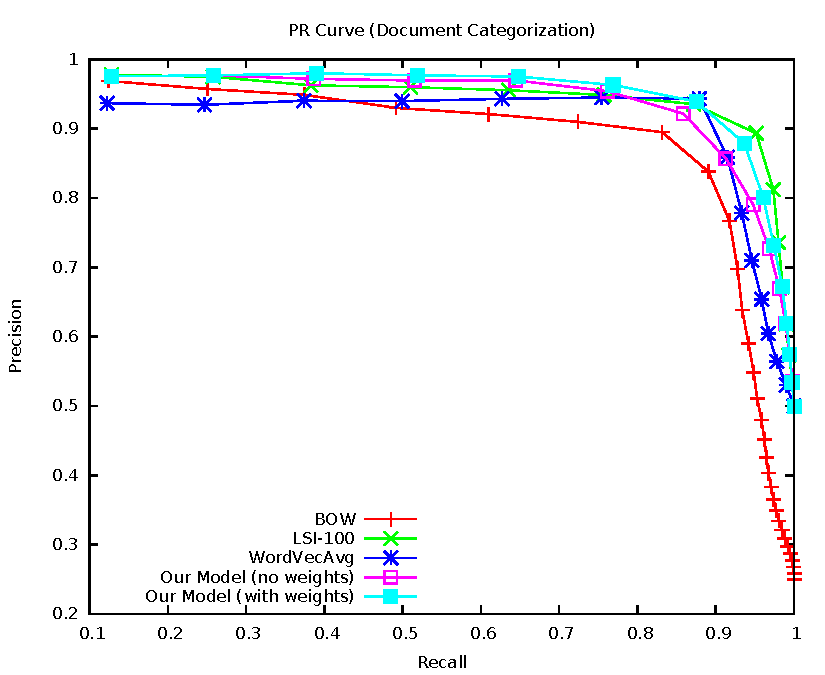
\includegraphics[scale=0.45]{../figs/pr/reuter-cs-scala.pdf}
		\end{figure}
	\end{center}
	\end{column}
}	
\end{columns}

\end{frame}

%%%%%%%%%%%%%%%%%%%%%%%%%%%%%%%%%%%%%%%%%%%%
\begin{frame}{Document Categorization Performance Evaluation \\ Physics - Wikipedia }
\begin{columns}[T]
	\hspace{5mm}
	\begin{column}{.4\textwidth}
		\begin{table}[h!]
		\tabcolsep=0.1cm
		\scriptsize
		\begin{center}
		\begin{tabular}{l@{\hskip5mm} c c@{\hskip4mm} c}
		\toprule
		% & \multicolumn{3}{c}{Reuters-21578}         \\
		% \cmidrule(lr){2-4}
		\textbf{Physics (Wikipedia)} & {P} & {R} & \textbf{F1} \\
		\midrule
		\textbf{BOW}
		& 87.8   & 70.1  & 77.9 \\
		\textbf{LSI-100}
		& 83.4   & 69.5  & 75.8 \\
		\textbf{WordVecAvg}
		& 91.0   & 59.1  & 71.7 \\ \addlinespace[1mm]

		\textbf{Our Model}
		& \multirow{2}{*}{86.1}   & \multirow{2}{*}{64.6}  & \multirow{2}{*}{73.8} \\
		(no weights) & & & \\ \addlinespace[1mm]
		\textbf{Our Model}
		& \multirow{2}{*}{88.6}   & \multirow{2}{*}{72.4}  & \multirow{2}{*}{\highest{79.7}} \\
		(with weights) & & & \\
		\bottomrule         
		\end{tabular}
		\caption*{\footnotesize Precision/Recall/F1 for Document Categorization on Physics dataset}
		\end{center}
		\end{table}
	\end{column}
	%\hspace{5mm}
\onslide<2->{	
	\begin{column}{.6\textwidth}
	\begin{center}
		\begin{figure}[tb]
		\centering
			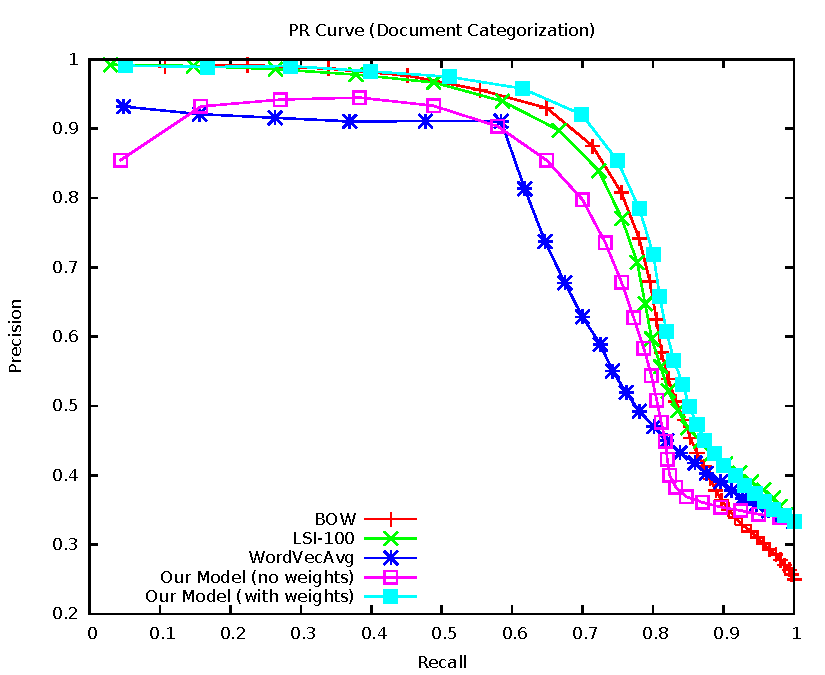
\includegraphics[scale=0.45]{../figs/pr/physics-cs-scala.pdf}
		\end{figure}
	\end{center}
	\end{column}
}	
\end{columns}

\end{frame}

%%%%%%%%%%%%%%%%%%%%%%%%%%%%%%%%%%%%%%%%%%%%
\begin{frame}{Document Categorization Performance Evaluation \\ Biology - Wikipedia }
\begin{columns}[T]
	\hspace{5mm}
	\begin{column}{.4\textwidth}
		\begin{table}[h!]
		\tabcolsep=0.1cm
		\scriptsize
		\begin{center}
		\begin{tabular}{l@{\hskip5mm} c c@{\hskip4mm} c}
		\toprule
		% & \multicolumn{3}{c}{Reuters-21578}         \\
		% \cmidrule(lr){2-4}
		\textbf{Biology (Wikipedia)} & {P} & {R} & \textbf{F1} \\
		\midrule
		\textbf{BOW}
		& 90.3   & 59.5  & \highest{69.0} \\
		\textbf{LSI-100}
		& 82.1   & 51.6  & 63.4 \\
		\textbf{WordVecAvg}
		& 79.4   & 50.4  & 61.6 \\ \addlinespace[1mm]

		\textbf{Our Model}
		& \multirow{2}{*}{80.3}   & \multirow{2}{*}{53.8}  & \multirow{2}{*}{64.4} \\
		(no weights) & & & \\ \addlinespace[1mm]
		\textbf{Our Model}
		& \multirow{2}{*}{79.7}   & \multirow{2}{*}{59.0}  & \multirow{2}{*}{67.8} \\
		(with weights) & & & \\
		\bottomrule         
		\end{tabular}
		\caption*{\footnotesize Precision/Recall/F1 for Document Categorization on Biology dataset}
		\end{center}
		\end{table}
	\end{column}
	%\hspace{5mm}
\onslide<2->{	
	\begin{column}{.6\textwidth}
	\begin{center}
		\begin{figure}[tb]
		\centering
			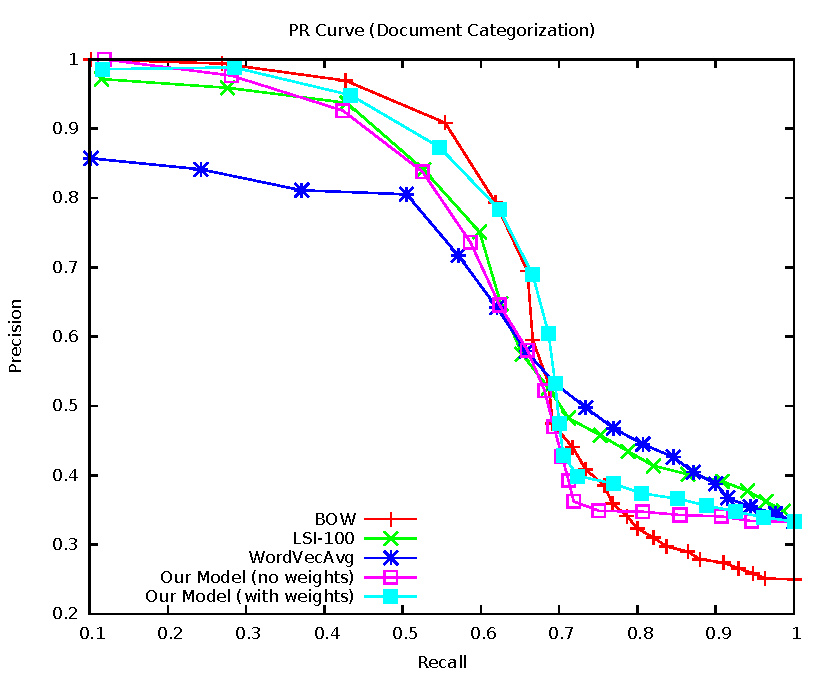
\includegraphics[scale=0.45]{../figs/pr/biology-cs-scala.pdf}
		\end{figure}
	\end{center}
	\end{column}
}	
\end{columns}

\end{frame}

%%%%%%%%%%%%%%%%%%%%%%%%%%%%%%%%%%%%%%%%%%%%
\begin{frame}{Document Categorization Performance Evaluation \\ Mathematics - Wikipedia }
\begin{columns}[T]
	\hspace{5mm}
	\begin{column}{.4\textwidth}
		\begin{table}[h!]
	\tabcolsep=0.1cm
	\scriptsize
	\begin{center}
	\begin{tabular}{l@{\hskip3mm} c c@{\hskip4mm} c}
	\toprule
	% & \multicolumn{3}{c}{Reuters-21578}         \\
	% \cmidrule(lr){2-4}
	\textbf{Mathematics (Wikipedia)} & {P} & {R} & \textbf{F1} \\
	\midrule
	\textbf{BOW}
	& 65.6   & 65.1  & 65.3 \\
	\textbf{LSI-100}
	& 89.7   & 50.3  & 64.4 \\
	\textbf{WordVecAvg}
	& 90.5   & 40.3  & 55.7 \\ \addlinespace[1mm]

	\textbf{Our Model}
	& \multirow{2}{*}{78.4}   & \multirow{2}{*}{57.4}  & \multirow{2}{*}{66.3} \\
	(no weights) & & & \\ \addlinespace[1mm]
	\textbf{Our Model}
	& \multirow{2}{*}{85.3}   & \multirow{2}{*}{56.8}  & \multirow{2}{*}{\highest{68.2}} \\
	(with weights) & & & \\
	\bottomrule         
	\end{tabular}
	%\vskip -4mm
	\caption*{\footnotesize Precision/Recall/F1 for Document Categorization on Mathematics dataset}
	\end{center}
	\end{table}
	\end{column}
	%\hspace{5mm}
\onslide<2->{	
	\begin{column}{.6\textwidth}
	\begin{center}
		\begin{figure}[tb]
		\centering
			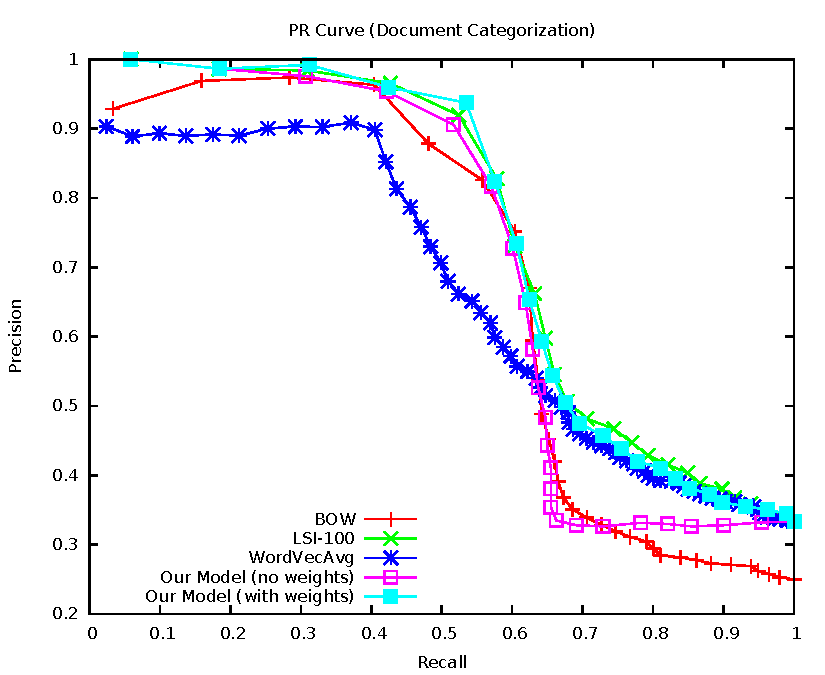
\includegraphics[scale=0.45]{../figs/pr/mathematics-cs-scala.pdf}
		\end{figure}
	\end{center}
	\end{column}
}	
\end{columns}

\end{frame}

%%%%%%%%%%%%%%%%%%%%%%%%%

\begin{frame}{Document Categorization Performance Evaluation \\ Sports - Wikipedia }
\begin{columns}[T]
	\hspace{5mm}
	\begin{column}{.4\textwidth}
		\vfill
		\begin{table}[h!]
		\tabcolsep=0.1cm
		\scriptsize
		\begin{center}
		\begin{tabular}{l@{\hskip5mm} c c@{\hskip4mm} c}
		\toprule
		% & \multicolumn{3}{c}{Reuters-21578}         \\
		% \cmidrule(lr){2-4}
		\textbf{Sports (Wikipedia)} & {P} & {R} & \textbf{F1} \\
		\midrule
		\textbf{BOW}
		& 91.7   & 41.3  & 56.9 \\
		\textbf{LSI-100}
		& 91.2   & 40.1  & 55.7 \\
		\textbf{WordVecAvg}
		& 81.8   & 37.5  & 51.4 \\ \addlinespace[1mm]

		\textbf{Our Model}
		& \multirow{2}{*}{80.5}   & \multirow{2}{*}{40.1}  & \multirow{2}{*}{53.6} \\
		(no weights) & & & \\ \addlinespace[1mm]
		\textbf{Our Model}
		& \multirow{2}{*}{82.1}   & \multirow{2}{*}{44.0}  & \multirow{2}{*}{\highest{57.3}} \\
		(with weights) & & & \\
		\bottomrule         
		\end{tabular}
		%\vskip -4mm
		\caption*{\footnotesize Precision/Recall/F1 for Document Categorization on Sports dataset}
		\end{center}
		\end{table}
	\end{column}
	%\hspace{5mm}
	
\onslide<2->{	
	\begin{column}{.6\textwidth}
	\vfill
	\begin{center}
		\begin{figure}[tb]
		\centering
			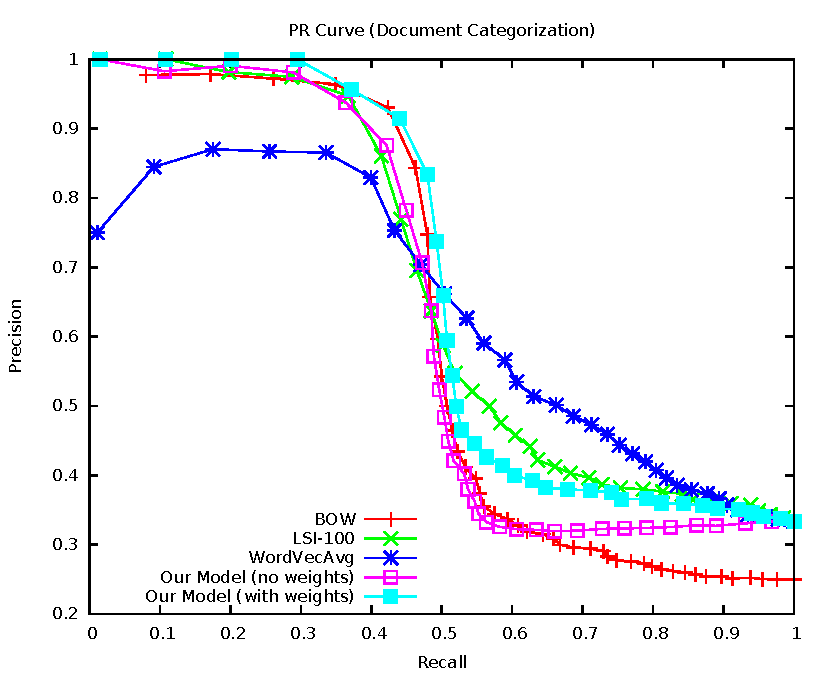
\includegraphics[scale=0.45]{../figs/pr/sports-cs-scala.pdf}
		\end{figure}
	\end{center}
	\end{column}
}	
\end{columns}

\end{frame}

%%%%%%%%%%%%%%%%%%%%%%%%%

\begin{frame}{Imputing Missing Categories in Wikipedia }
\begin{enumerate}
	\vfill\item Real-life databases contain missing information
	\vfill\item Wikipedia is a large-scale database with non-expert annotators
\end{enumerate}
\vfill
We evaluate our model on imputing missing categories in the Wikipedia datasets
\vfill
	\begin{table}[h!]
	\tabcolsep=1mm
	\tiny
	\begin{center}
	%\begin{tabular}{l cc@{\hskip 2mm}c@{\hskip 2mm} cc@{\hskip 2mm}c@{\hskip 2mm} cc@{\hskip 2mm}c@{\hskip 2mm} cc@{\hskip 2mm}c@{\hskip 2mm} cc@{\hskip 2mm}c}
	\begin{tabular}{l ccc@{\hskip 3mm} ccc@{\hskip 3mm} ccc@{\hskip 3mm} ccc@{\hskip 3mm} ccc}
	\toprule
	\multirow{2}{*}{} & 
	\multicolumn{3}{c}{{Physics}}         & 
	\multicolumn{3}{c}{{Biology}}        & \multicolumn{3}{c}{{Mathematics}}         & \multicolumn{3}{c}{{Sports}}        & %\multicolumn{3}{c}{\textbf{Restaurant}}       & 
	\multicolumn{3}{c}{\textbf{Combined}}              
	\\ 
	\cmidrule(lr){2-4}
	\cmidrule(lr){5-7}
	\cmidrule(lr){8-10}
	\cmidrule(lr){11-13}
	\cmidrule(lr){14-16}
	& 
	{P} & {R} & \textbf{F1} & 
	{P} & {R} & \textbf{F1} & 
	{P} & {R} & \textbf{F1} & 
	{P} & {R} & \textbf{F1} &
	{P} & {R} & \textbf{F1} \\ 
	\midrule
	\textbf{PMF}
	& 73.0   & 64.3  & 68.4
	& 72.1   & 47.5  & 57.3
	& 41.6   & 58.2  & 48.5
	& 51.3   & 35.6  & 42.0
	& 63.0   & 54.8  & 58.6 
	\\
	\textbf{LSI-100}
	& 59.5   & 82.3  & 69.0
	& 49.9   & 71.6  & 58.8
	& 47.1   & 73.0  & 57.3
	& 43.1   & 68.2  & 52.8
	& 52.5   & 76.3  & 62.2
	\\ 
	\textbf{BOW}
	& 76.1   & 79.4  & 77.7
	& 69.7   & 67.7  & 68.7
	& 70.9   & 63.5  & 67.0
	& 64.8   & 49.3  & 56.0
	& 72.5   & 69.4  & 70.9
	\\
	\textbf{WordVecAvg}
	& 88.0   & 63.5  & 73.8
	& 80.7   & 50.3  & 61.9
	& 71.8   & 46.7  & 56.6
	& 87.2   & 35.4  & 50.3
	& 84.2   & 53.4  & 65.4
	\\ \addlinespace[1mm]
	\textbf{Our Model}
	& \multirow{2}{*}{88.6}   & \multirow{2}{*}{69.1}  & \multirow{2}{*}{77.7}
	& \multirow{2}{*}{80.5}   & \multirow{2}{*}{55.3}  & \multirow{2}{*}{65.6}
	& \multirow{2}{*}{74.3}   & \multirow{2}{*}{53.1}  & \multirow{2}{*}{61.9}
	& \multirow{2}{*}{84.7}   & \multirow{2}{*}{40.2}  & \multirow{2}{*}{54.5}
	& \multirow{2}{*}{85.4}   & \multirow{2}{*}{58.5}  & \multirow{2}{*}{69.2}
	\\ 
	(without weights) & & & & & & & & & & & & & &  & \\
	\addlinespace[1mm]
	\textbf{Our Model}
	& \multirow{2}{*}{89.9}   & \multirow{2}{*}{74.5}  & \multirow{2}{*}{\highest{81.5}}
	& \multirow{2}{*}{84.9}   & \multirow{2}{*}{63.8} & \multirow{2}{*}{\highest{72.9}}
	& \multirow{2}{*}{79.9}   & \multirow{2}{*}{60.7}  & \multirow{2}{*}{\highest{69.0}}
	& \multirow{2}{*}{81.1}   & \multirow{2}{*}{45.6} & \multirow{2}{*}{\highest{58.4}}
	& \multirow{2}{*}{86.3}   & \multirow{2}{*}{65.2}  & \multirow{2}{*}{\highest{74.3}}
	\\ 
	(with weights) & & & & & & & & & & & & & &  & \\
	\bottomrule         
	\end{tabular}
	\end{center}
	\end{table}


\end{frame}

\begin{frame}{Estimating Similarity between Categories and Words }
\begin{enumerate}
	\vfill\item We embed words, document and categories in the same $k$-dimensional space
	\vfill\item This allows us to estimate similarity between entities non directly related
\end{enumerate}
\begin{table}[h!]
\tabcolsep=1mm
\scriptsize
\begin{center}
%\begin{adjustwidth}{-1.5cm}{}
\begin{tabular}{l@{\hskip3mm} l}
\toprule
\multirow{2}{*}{\textbf{Category}} & \multirow{2}{*}{\textbf{Nearest Neighbors}} \\
 & \\
%\cmidrule{2-2}
\textbf{Evolutionary Biology}   & gene, phylogenetics, speciation, ancestor, Darwin, lineage, evolutionary, interbreeding \\
\textbf{Statistical Mechanics}  & ergodicity, Eigenstate, Universality, DMFT, Markovian, Parisi, Combinatorics \\
\textbf{Thermodynamics}         & Convection, ecosystem, Enthalpy, Joule, calorimetric, compressible, Thermodynamic \\
\textbf{Trade}                  & import, Pledges, Tariff, Trade, competitiveness, toll, billion, basket, Ditch, Worldwide \\
\textbf{Money-FX}               & Borrowing, franc, banker, Currency, banks, nervous, sideways, Markets, FORWARD \\
\textbf{Virology}               & nucleoside, ribozyme, adenoviruses, Virology, retroviruses, poliovirus, Viroid \\
\textbf{Neurobiology}           & purinergic, cyclase, vertebral, Ehrlich, nexus, steroid, lean, gendered, reticular \\
\textbf{Physical Exercise}      & Fitness, aerobics, metabolic, workout, Exercise, Stretching, pelvic, Physiology, fibers \\
\textbf{Algebra}                & subalgebra, Algebras, nilpotent, adjoints, octonions, bicommutant, diagonalizable \\
\textbf{Theoretical Physicists} & Dipankar, DSc, Hubert, Aneesur, Uri, Ignaz, Chia, Stig, Diderot, Dannie \\
\textbf{Mathematical Physics}   & covectors, pseudotensor, spacelike, dyadic, Curl, torque, contractions, wavefunctions \\
\textbf{Sports Venues}          & stadion, decoration, tracks, seating, buildings, parcourse, architectural, arenas, circular \\
\textbf{Indian Mathematics}     & utkrama, ecliptic, Siddhanta, Hellenistic, Brahmi, sexagesimal, scribe, Islamic, Sanskrit \\
\bottomrule         
\end{tabular}
 %\end{adjustwidth}
\end{center}
%\caption{\label{catword:sim} Estimating Similarity between Categories and Words}
\end{table}
\end{frame}

\begin{frame}{Conclusion }
\begin{enumerate}
	\vfill\item<1-> We presented an unsupervised neural network model that 
	\begin{itemize}
		\vfill\item Jointly learns fixed-length low-dimensional distributed vector representations for documents and words
		\vfill\item Encode semantic content of words and documents in these representations
	\end{itemize}
	
	\vfill\item<2-> We overcome some of the problems with the bag-of-words representations 
	\vfill\item<3-> Our model is a log-linear model that uses NCE
	\vfill\item<4-> We improve state-of-the-art results on multi-label document categorization
	\begin{itemize}
		\vfill\item On the Reuters-21578 dataset we improve by $3.26\%$
		\vfill\item On the Reuters-21578 dataset we improve over BOW by $9\%$
	\end{itemize}
	\vfill\item<5-> We show the best performance on imputing missing categories in Wikipedia
	\vfill\item<6-> Learned distributed representations allow semantic similarity estimation
\end{enumerate}
\end{frame}

\begin{frame}{Future Work }
\begin{enumerate}
	\item<1-> Improving compositionality of Word Vectors
	\vfill\item<2-> Joint Document Representation Learning and Document Categorization
	\vfill\item<3-> Supervised Multi-view Relational Learning
\end{enumerate}

\end{frame}

%%%%%%%%%%%%%%%%%%%%%%%%%%%%%%%%%%%%%%%%%%%
\begin{frame}[allowframebreaks]{References}
    %{\footnotesize
    \scriptsize
    \bibliographystyle{abbrvnat}
    \bibliography{references}
    %}
\end{frame}

\begin{frame}
\vfill
\begin{center}
\Large Thank You! 
\\
\large Questions?
\end{center}
\blfootnote{Snacks outside}
\end{frame}


\end{document}